\section{Resultados}

Los resultados se presentan en dos partes. La Parte~I aborda el an\'alisis de transferencia de calor: c\'alculo detallado paso a paso del coeficiente global $U$, simulaci\'on transitoria del calentamiento para los cuatro escenarios definidos, an\'alisis del ciclo de descargas a carrotanque, y dimensionamiento del aislamiento t\'ermico. La Parte~II presenta el an\'alisis estructural del tanque seg\'un API~650 y ASME~VIII con desarrollo num\'erico completo.

\subsection{Parte I: An\'alisis de Transferencia de Calor}

\subsubsection{Coeficiente Global de Transferencia de Calor}

El coeficiente global $U$ se calcul\'o mediante el modelo de resistencias en serie (Ec.~\ref{eq:U_global}). La resistencia del lado del agua se determin\'o con la correlaci\'on de Sieder-Tate para flujo turbulento, y la resistencia del lado de la glucosa con la correlaci\'on de Churchill-Chu para convecci\'on natural. La Tabla~\ref{tab:U_results} resume los resultados para los Escenarios~2 y 3 a diferentes temperaturas de la glucosa.

\begin{table}[H]
	\centering
	\caption{Coeficiente global $U$ y par\'ametros de transferencia de calor para los Escenarios~2 y~3 ($v_w = 2.5$~m/s).}
	\label{tab:U_results}
	\setcounter{itemcount}{0}
	\begin{tabularx}{\textwidth}{@{}NccccccX@{}}
		\toprule
		\multicolumn{1}{c}{\textbf{Item}} & $T_g$ [°C] & $T_w$ [°C] & $h_i$ [W/m\textsuperscript{2}°C] & $h_o$ [W/m\textsuperscript{2}°C] & $U$ [W/m\textsuperscript{2}°C] & Re & \textbf{$R_o/R_T$ [\%]} \\
		\midrule
		& 20 & 65 & 10\,226 & 18.2 & 17.9 & 392\,000 & 98.8 \\
		& 30 & 65 & 10\,356 & 22.6 & 22.3 & 392\,000 & 98.6 \\
		& 40 & 65 & 10\,480 & 26.5 & 26.0 & 392\,000 & 98.3 \\
		& 50 & 65 & 10\,599 & 28.5 & 28.0 & 392\,000 & 98.2 \\
		& 60 & 65 & 10\,713 & 25.0 & 24.6 & 392\,000 & 98.4 \\
		\midrule
		& 20 & 75 & 10\,867 & 21.4 & 21.1 & 448\,000 & 98.6 \\
		& 30 & 75 & 10\,997 & 26.7 & 26.3 & 448\,000 & 98.3 \\
		& 40 & 75 & 11\,122 & 31.7 & 31.1 & 448\,000 & 98.0 \\
		& 50 & 75 & 11\,241 & 35.7 & 34.9 & 448\,000 & 97.8 \\
		& 60 & 75 & 11\,356 & 37.1 & 36.2 & 448\,000 & 97.7 \\
		\bottomrule
	\end{tabularx}
\end{table}

Los resultados confirman que el coeficiente del lado del agua ($h_i \approx 10\,200$--$11\,400$~W/m\textsuperscript{2}$\cdot$°C) es entre 290 y 610 veces mayor que el coeficiente del lado de la glucosa ($h_o \approx 18$--$37$~W/m\textsuperscript{2}$\cdot$°C). La resistencia t\'ermica del lado de la glucosa representa entre el 97.7\% y el 98.8\% de la resistencia total, lo que indica que el mecanismo limitante de la transferencia de calor es la convecci\'on natural de la glucosa, severamente restringida por la viscosidad de 212\,000~cP a 20~°C (ficha t\'ecnica Ingredion~011420). Incrementar el caudal o la turbulencia del agua en la media ca\~na no produce mejora apreciable sobre $U$.

\subsubsection{Desarrollo Num\'erico Detallado del Coeficiente $U$}

Se presenta a continuaci\'on el c\'alculo paso a paso del coeficiente global de transferencia de calor para la condici\'on representativa del Escenario~3: $T_g = 40$~°C, $T_w = 75$~°C, $v_w = 2.5$~m/s.

\textbf{Paso 1: Di\'ametro hidr\'aulico de la media ca\~na.} El canal rectangular de la media ca\~na tiene dimensiones internas $a = 141$~mm y $b = 45.5$~mm. El di\'ametro hidr\'aulico se calcula seg\'un la Ec.~\ref{eq:Dh}:

\begin{equation}
	D_h = \frac{4 \cdot A_c}{P_m} = \frac{4 \times (0.141 \times 0.0455)}{2 \times (0.141 + 0.0455)} = \frac{4 \times 6.4155 \times 10^{-3}}{0.373} = 0.0688~\text{m} = 68.8~\text{mm}
\end{equation}

\textbf{Paso 2: Propiedades del agua a 75~°C.} Las propiedades termof\'isicas del agua a la temperatura del fluido de calentamiento se eval\'uan mediante las correlaciones del m\'odulo de c\'alculo:

\begin{equation}
\begin{aligned}
	\rho_w &= 975.1~\text{kg/m}^3, \quad \mu_w = 3.74 \times 10^{-4}~\text{Pa} \cdot \text{s}, \quad C_{p,w} = 4\,160~\text{J/(kg} \cdot \text{°C)} \\
	k_w &= 0.667~\text{W/(m} \cdot \text{°C)}, \quad \text{Pr}_w = \frac{C_{p,w} \cdot \mu_w}{k_w} = \frac{4160 \times 3.74 \times 10^{-4}}{0.667} = 2.34
\end{aligned}
\end{equation}

\textbf{Paso 3: N\'umero de Reynolds.} Con la velocidad del agua $v = 2.5$~m/s en la media ca\~na:

\begin{equation}
	\text{Re} = \frac{\rho_w \cdot v \cdot D_h}{\mu_w} = \frac{975.1 \times 2.5 \times 0.0688}{3.74 \times 10^{-4}} = 448\,000 \gg 10\,000 \quad \text{(flujo turbulento)}
\end{equation}

\textbf{Paso 4: N\'umero de Nusselt del agua (Sieder-Tate).} La temperatura estimada de la pared es $T_{pared} \approx (T_w + T_g)/2 = (75+40)/2 = 57.5$~°C. La viscosidad del agua a la temperatura de pared es $\mu_w|_{T_p} = 4.81 \times 10^{-4}$~Pa$\cdot$s. Se aplica la Ec.~\ref{eq:sieder_tate}:

\begin{equation}
\begin{aligned}
	\text{Nu} &= 0.027 \times \text{Re}^{0.8} \times \text{Pr}^{1/3} \times \left(\frac{\mu}{\mu_w}\right)^{0.14} \\
	&= 0.027 \times (448\,000)^{0.8} \times (2.34)^{1/3} \times \left(\frac{3.74 \times 10^{-4}}{4.81 \times 10^{-4}}\right)^{0.14} \\
	&= 0.027 \times 33\,194 \times 1.327 \times 0.965 \\
	&= 1\,148
\end{aligned}
\end{equation}

\textbf{Paso 5: Coeficiente del lado del agua ($h_i$).}

\begin{equation}
	h_i = \frac{\text{Nu} \cdot k_w}{D_h} = \frac{1\,148 \times 0.667}{0.0688} = 11\,122~\text{W/(m}^2 \cdot \text{°C)}
\end{equation}

\textbf{Paso 6: Propiedades de la glucosa a $T_{film}$.} La temperatura de pel\'icula del lado de la glucosa es $T_f = (T_{pared} + T_g)/2 = (57.5 + 40)/2 = 48.75$~°C. Las propiedades de la glucosa Globe~42~DE a esta temperatura se eval\'uan mediante la correlaci\'on VFT (Ec.~\ref{eq:vft}) para la viscosidad y las correlaciones de Choi~\&~Okos para $C_p$ y $k$:

\begin{equation}
\begin{aligned}
	\rho_g &= 1435.4 - 0.540 \times 48.75 = 1\,409.1~\text{kg/m}^3 \\
	\mu_g &= \exp\!\left(-9.350 + \frac{1\,278.0}{48.75 + 66.90}\right) = \exp(1.701) = 5.48~\text{Pa} \cdot \text{s} = 5\,478~\text{cP} \\
	C_{p,g} &= 2\,123~\text{J/(kg} \cdot \text{°C)}, \quad k_g = 0.333~\text{W/(m} \cdot \text{°C)} \\
	\beta_g &= \frac{0.540}{1\,409.1} = 3.83 \times 10^{-4}~\text{°C}^{-1}
\end{aligned}
\end{equation}

\textbf{Paso 7: N\'umero de Rayleigh de la glucosa.} La longitud caracter\'istica para la convecci\'on natural sobre el fondo toriesf\'erico se estima como $L = 1.0$~m, y la diferencia de temperatura es $\Delta T = T_{pared} - T_g = 57.5 - 40 = 17.5$~°C:

\begin{equation}
\begin{aligned}
	\nu_g &= \frac{\mu_g}{\rho_g} = \frac{5.48}{1\,409.1} = 3.89 \times 10^{-3}~\text{m}^2\text{/s} \\
	\alpha_g &= \frac{k_g}{\rho_g \cdot C_{p,g}} = \frac{0.333}{1\,409.1 \times 2\,123} = 1.11 \times 10^{-7}~\text{m}^2\text{/s} \\
	\text{Gr} &= \frac{g \cdot \beta_g \cdot \Delta T \cdot L^3}{\nu_g^2} = \frac{9.81 \times 3.83 \times 10^{-4} \times 17.5 \times 1.0^3}{(3.89 \times 10^{-3})^2} = 4.35 \times 10^{3} \\
	\text{Ra} &= \text{Gr} \times \text{Pr}_g = 4.35 \times 10^{3} \times 34\,894 = 1.52 \times 10^{8}
\end{aligned}
\end{equation}

donde $\text{Pr}_g = \mu_g \cdot C_{p,g} / k_g = 5.48 \times 2\,123 / 0.333 = 34\,894$. El extraordinario valor del n\'umero de Prandtl refleja la dominancia de la difusi\'on viscosa sobre la difusi\'on t\'ermica en la glucosa a 80.6~°Brix, lo que limita severamente la convecci\'on natural.

\textbf{Paso 8: N\'umero de Nusselt de la glucosa (Churchill-Chu).} Se aplica la Ec.~\ref{eq:churchill_chu}:

\begin{equation}
\begin{aligned}
	\text{Nu}_L &= \left[0.825 + \frac{0.387 \times \text{Ra}^{1/6}}{\left(1 + (0.492/\text{Pr})^{9/16}\right)^{8/27}}\right]^2 \\
	&= \left[0.825 + \frac{0.387 \times (1.52 \times 10^{8})^{1/6}}{\left(1 + (0.492/34\,894)^{9/16}\right)^{8/27}}\right]^2 \\
	&= \left[0.825 + \frac{0.387 \times 23.1}{(1.000)^{8/27}}\right]^2 \\
	&= \left[0.825 + 8.94\right]^2 = 95.2
\end{aligned}
\end{equation}

\textbf{Paso 9: Coeficiente del lado de la glucosa ($h_o$).}

\begin{equation}
	h_o = \frac{\text{Nu}_L \cdot k_g}{L} = \frac{95.2 \times 0.333}{1.0} = 31.7~\text{W/(m}^2 \cdot \text{°C)}
\end{equation}

\textbf{Paso 10: Coeficiente global $U$.} Sustituyendo en la Ec.~\ref{eq:U_global} con $e_w = 9$~mm y $k_{SS} = 16.3$~W/(m$\cdot$°C):

\begin{equation}
\begin{aligned}
	\frac{1}{U} &= \frac{1}{h_i} + \frac{e_w}{k_{SS}} + \frac{1}{h_o} = \frac{1}{11\,122} + \frac{0.009}{16.3} + \frac{1}{31.7} \\
	&= 9.0 \times 10^{-5} + 5.52 \times 10^{-4} + 3.15 \times 10^{-2} = 3.22 \times 10^{-2}~\text{m}^2 \cdot \text{°C/W}
\end{aligned}
\end{equation}

\begin{equation}
	\boxed{U = \frac{1}{3.22 \times 10^{-2}} = 31.1~\text{W/(m}^2 \cdot \text{°C)}}
\end{equation}

\textbf{Paso 11: Distribuci\'on de resistencias t\'ermicas.}

\begin{equation}
\begin{aligned}
	\%R_i &= \frac{1/h_i}{1/U} \times 100 = \frac{9.0 \times 10^{-5}}{3.22 \times 10^{-2}} \times 100 = 0.3\% \quad \text{(agua)} \\
	\%R_w &= \frac{e_w/k_{SS}}{1/U} \times 100 = \frac{5.52 \times 10^{-4}}{3.22 \times 10^{-2}} \times 100 = 1.7\% \quad \text{(pared)} \\
	\%R_o &= \frac{1/h_o}{1/U} \times 100 = \frac{3.15 \times 10^{-2}}{3.22 \times 10^{-2}} \times 100 = \textbf{98.0\%} \quad \text{(glucosa)}
\end{aligned}
\end{equation}

El resultado confirma que la resistencia del lado de la glucosa domina de forma abrumadora el proceso de transferencia de calor (98.0\%), relegando la resistencia de la pared de SS316L al 1.7\% y la del agua al 0.3\%. La viscosidad de la glucosa Globe~42~DE a 80.6~°Brix ($> 5\,400$~cP a la temperatura de pel\'icula) genera un n\'umero de Prandtl del orden de $10^4$, lo que restringe severamente la convecci\'on natural y explica los prolongados tiempos de calentamiento reportados.

\subsubsection{Escenario 1: Volumen Parcial (24~m\textsuperscript{3})}

El Escenario~1 eval\'ua el calentamiento de un volumen parcial de 24~m\textsuperscript{3} de glucosa (34.1~toneladas) con un caudal de agua de 30.9~m\textsuperscript{3}/h (velocidad en la media ca\~na de 1.34~m/s, temperatura del agua de 65~°C). Este escenario permite caracterizar el comportamiento t\'ermico del sistema con una carga parcial del tanque.

La simulaci\'on transitoria arroj\'o un tiempo de calentamiento de 20~°C a 60~°C de \textbf{132.0~horas}. A pesar de tratarse de un volumen parcial (24~m\textsuperscript{3}, 34.2~toneladas), el tiempo resulta considerable debido a la alt\'isima viscosidad de la glucosa a temperaturas inferiores a 40~°C ($> 13\,500$~cP), que restringe severamente el coeficiente de convecci\'on natural en el lado del producto.

Al alcanzar la temperatura de descarga de 60~°C, se model\'o la descarga de 24~toneladas de glucosa en 1.5~horas por la boquilla de 8''. La velocidad de descarga en la boquilla resulta $v_{8''} = 0.098$~m/s. Durante la descarga, el sistema de calentamiento contin\'ua operando; la temperatura de la glucosa se incrementa ligeramente de 60.0~°C a 60.9~°C debido a que la masa en el tanque disminuye (mejorando la relaci\'on \'area/masa) mientras el flujo de calor se mantiene. La Figura~\ref{fig:escenario1} presenta el perfil de temperatura y la evoluci\'on de la masa durante ambas fases.

\begin{figure}[H]
	\centering
	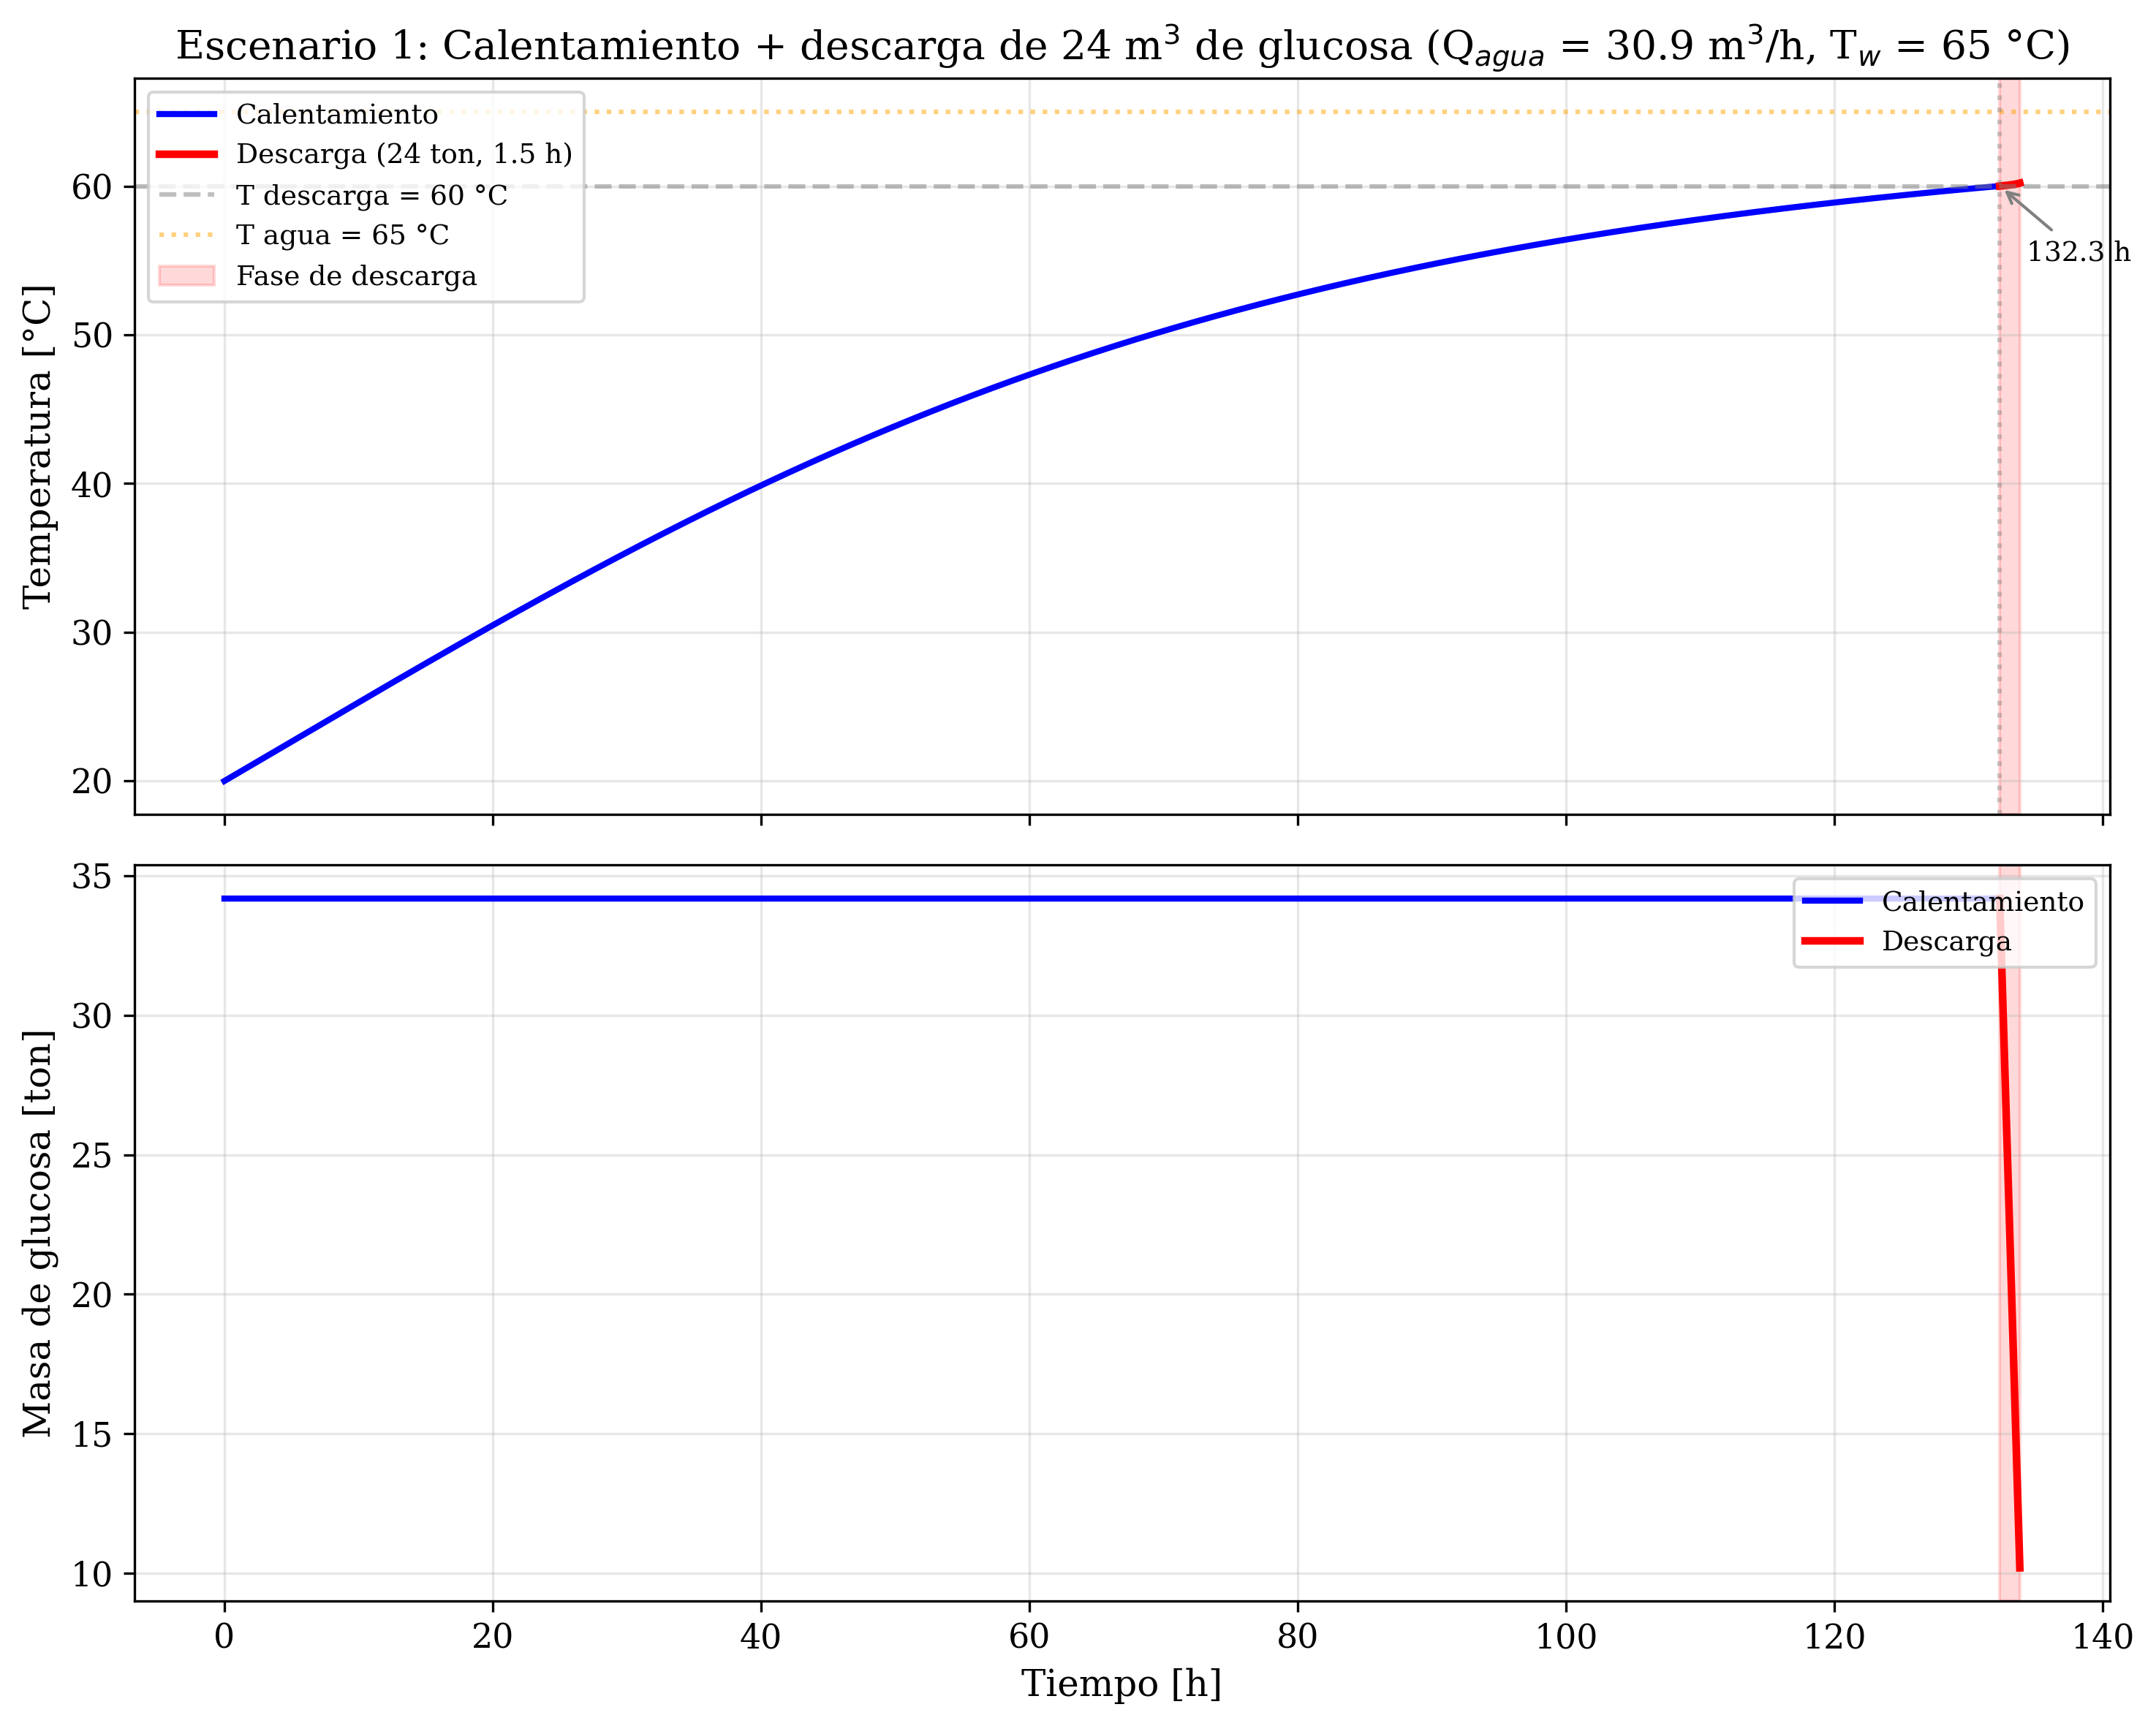
\includegraphics[width=0.95\textwidth]{../figures/escenario1_T_vs_tiempo.png}
	\caption{Escenario 1: Calentamiento y descarga de 24~m\textsuperscript{3} de glucosa ($Q_w$ = 30.9~m\textsuperscript{3}/h, $T_{w,in}$ = 65~°C). Panel superior: temperatura de la glucosa. Panel inferior: masa de glucosa en el tanque. La zona sombreada indica la fase de descarga.}
	\label{fig:escenario1}
\end{figure}

\subsubsection{Escenario 2: Tanque al 80\%, Agua a 65~°C}

El Escenario~2 representa la condici\'on m\'as exigente: el tanque al 80\% de su capacidad (178.2~m\textsuperscript{3}, equivalentes a 253~toneladas) con agua de calentamiento a 65~°C y velocidad de 2.5~m/s en la media ca\~na. La Tabla~\ref{tab:tiempos_esc2} resume los tiempos de calentamiento.

\begin{table}[H]
	\centering
	\caption{Tiempos de calentamiento -- Escenario 2 (tanque al 80\%, $T_{w,in}$ = 65~°C, $v_w$ = 2.5~m/s).}
	\label{tab:tiempos_esc2}
	\setcounter{itemcount}{0}
	\begin{tabularx}{0.85\textwidth}{@{}NccX@{}}
		\toprule
		\multicolumn{1}{c}{\textbf{Item}} & \textbf{$T$ objetivo [°C]} & \textbf{Tiempo [h]} & \textbf{Observaci\'on} \\
		\midrule
		& 30 & 142.0 & Viscosidad a\'un muy alta (46\,500~cP) \\
		& 40 & 299.0 & Inicio de fluidez moderada (13\,500~cP) \\
		& 50 & 512.5 & Viscosidad 4\,870~cP \\
		& 55 & 678.5 & -- \\
		& 57 & 772.8 & Temperatura operativa de descarga \\
		& 60 & 981.6 & L\'imite m\'aximo permisible (recomendaci\'on de corte) \\
		\bottomrule
	\end{tabularx}
\end{table}

Los resultados revelan que, con agua a 65~°C, alcanzar la temperatura operativa de descarga de 57~°C requiere \textbf{772.8~horas de calentamiento continuo}. Este extenso transcurso obedece a la enorme viscosidad de la glucosa a 80.6~°Brix ($> 212{,}000$~cP a 20~°C, ficha t\'ecnica Ingredion~011420), que estrangula severamente la convecci\'on natural y reduce el coeficiente de transferencia del lado del producto. Con respecto a la cota cr\'itica de los $60^\circ\mathrm{C}$, esta se alcanzar\'ia a los 981.6~horas, raz\'on por la cual se recomienda instrumentar un lazo de control que suspenda el suministro t\'ermico al alcanzar dicho umbral. La Figura~\ref{fig:escenario2} presenta el perfil de temperatura.

\begin{figure}[H]
	\centering
	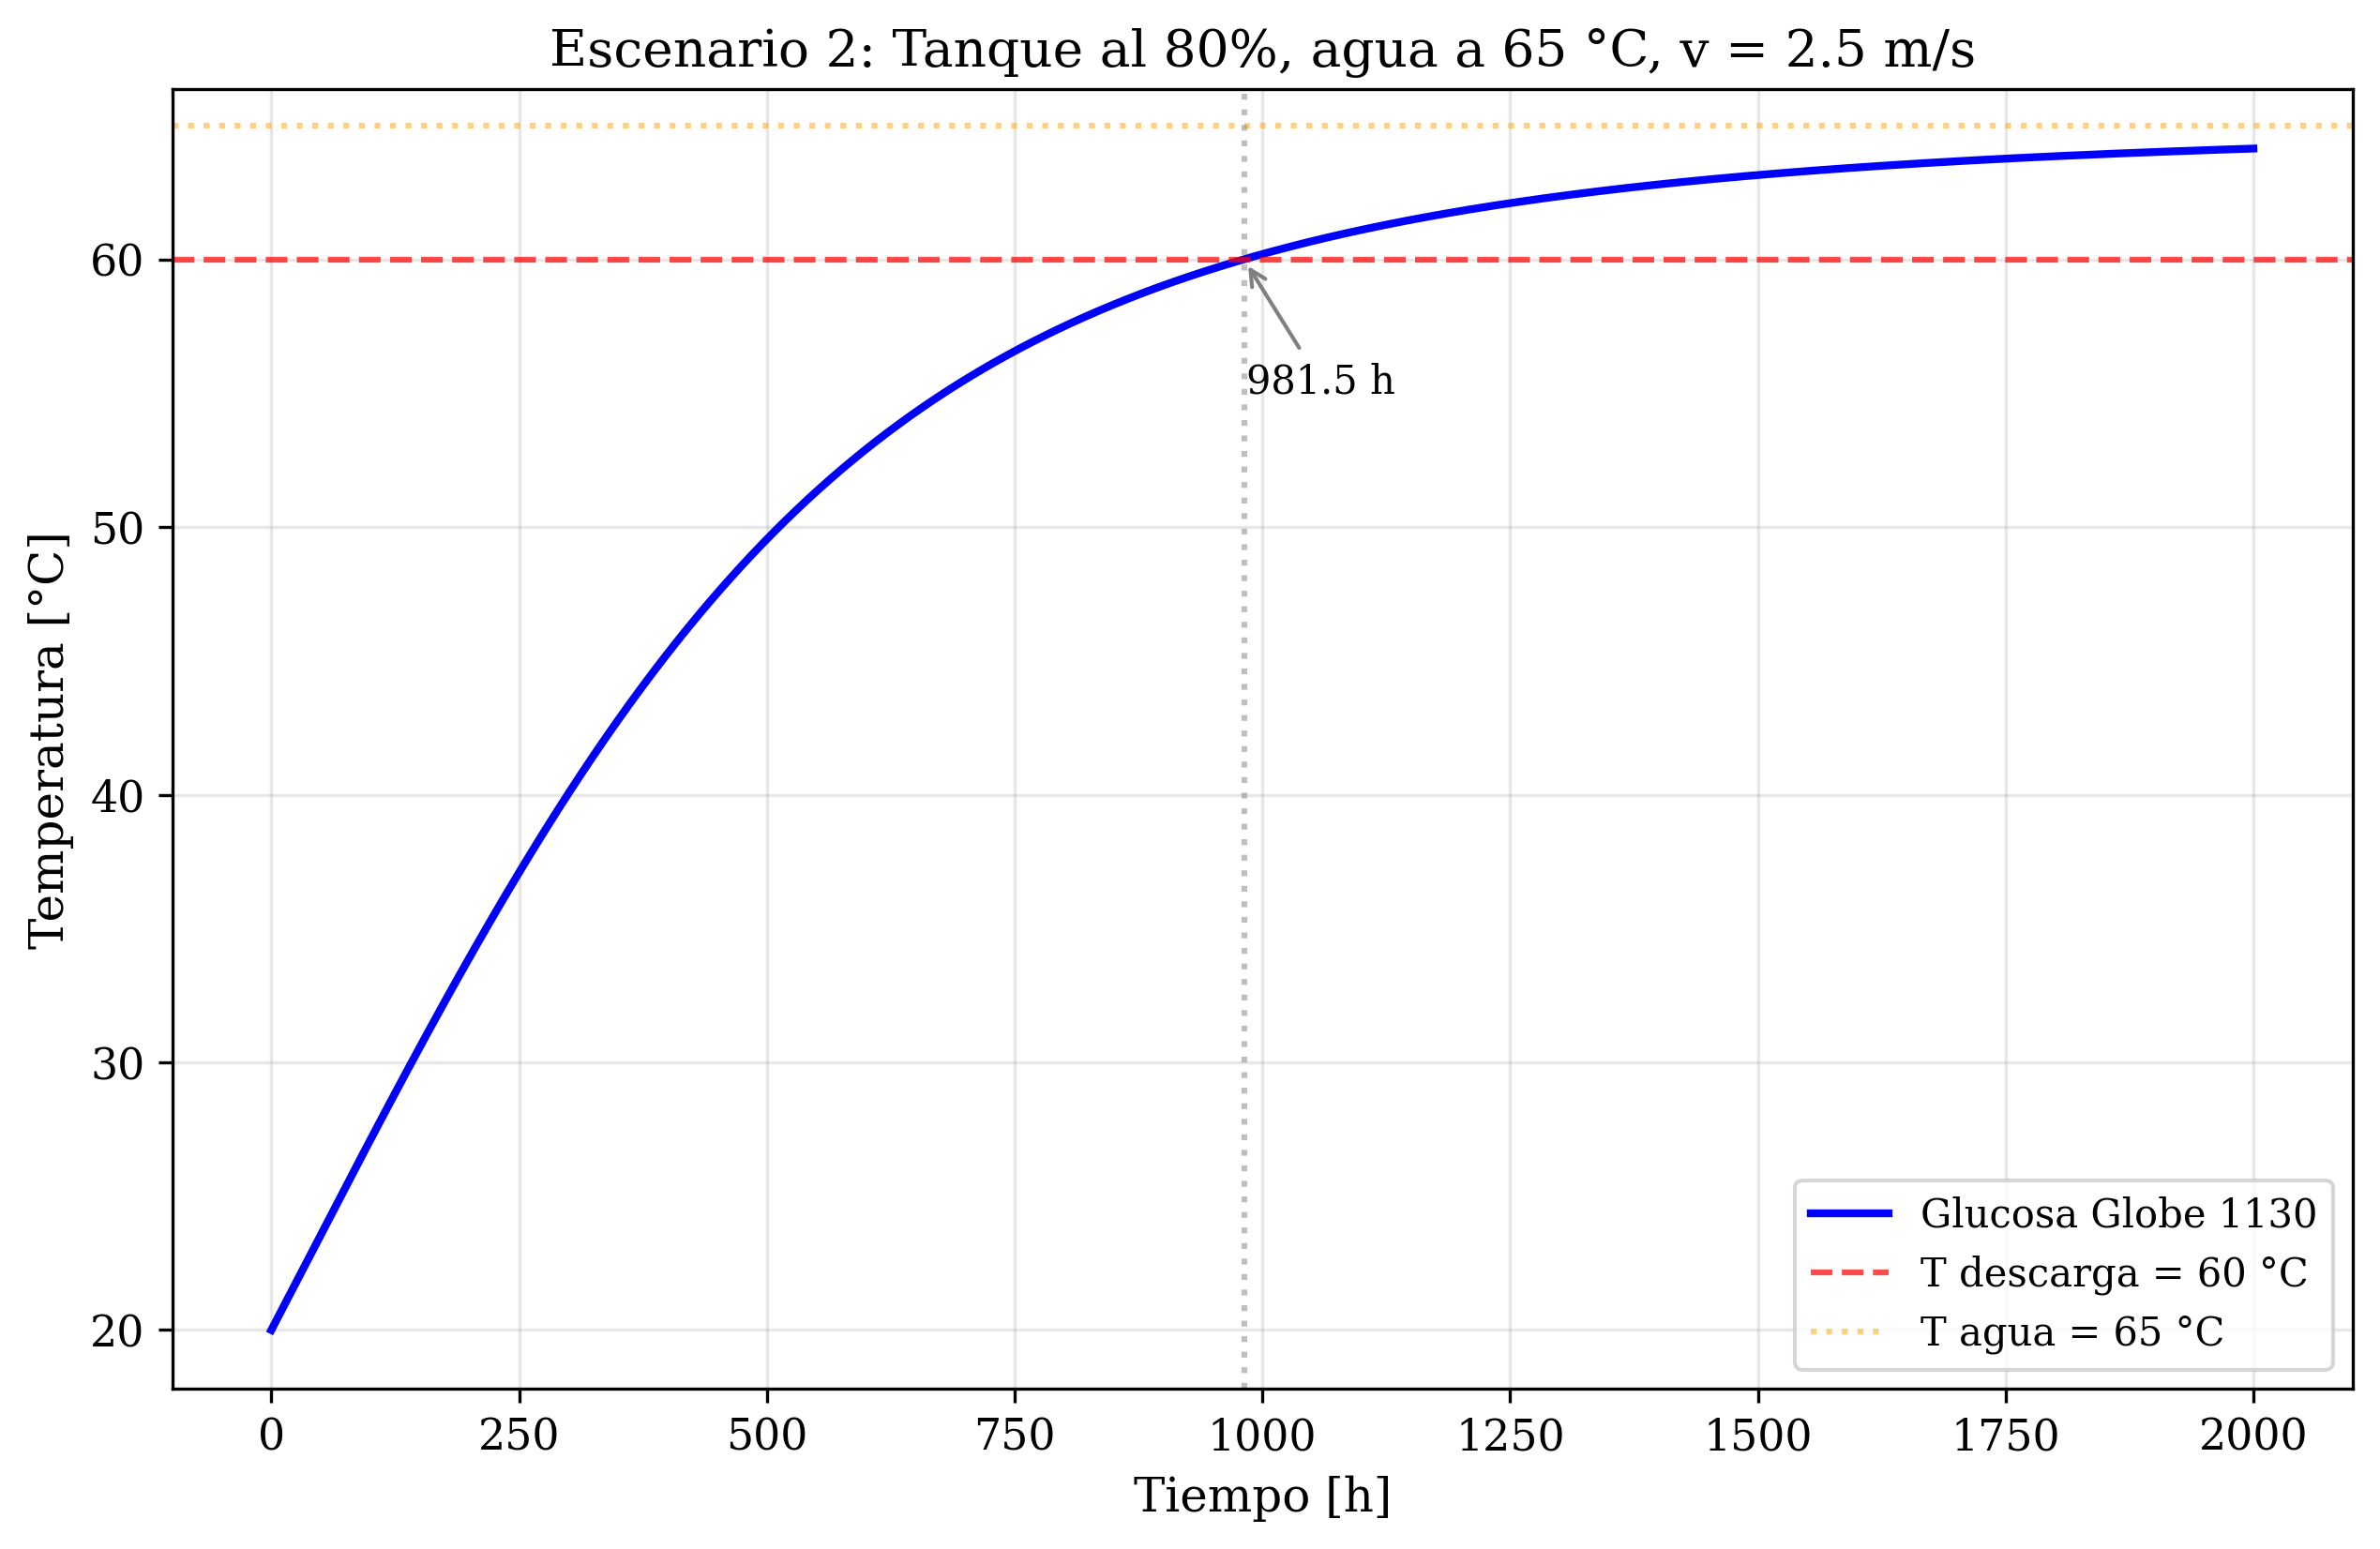
\includegraphics[width=0.85\textwidth]{../figures/escenario2_T_vs_tiempo.png}
	\caption{Escenario 2: Perfil de temperatura de la glucosa durante el calentamiento del tanque al 80\% ($T_{w,in}$ = 65~°C, $v_w$ = 2.5~m/s).}
	\label{fig:escenario2}
\end{figure}

\subsubsection{Escenario 3: Tanque al 80\%, Agua a 75~°C}

El Escenario~3 es id\'entico al Escenario~2, excepto que la temperatura del agua de entrada se incrementa a 75~°C. Los tiempos de calentamiento se presentan en la Tabla~\ref{tab:tiempos_esc3}.

\begin{table}[H]
	\centering
	\caption{Tiempos de calentamiento -- Escenario 3 (tanque al 80\%, $T_{w,in}$ = 75~°C, $v_w$ = 2.5~m/s).}
	\label{tab:tiempos_esc3}
	\setcounter{itemcount}{0}
	\begin{tabularx}{0.85\textwidth}{@{}NccX@{}}
		\toprule
		\multicolumn{1}{c}{\textbf{Item}} & \textbf{$T$ objetivo [°C]} & \textbf{Tiempo [h]} & \textbf{Observaci\'on} \\
		\midrule
		& 30 & 96.5 & -- \\
		& 40 & 196.0 & -- \\
		& 50 & 311.0 & -- \\
		& 55 & 383.0 & -- \\
		& 57 & 415.2 & Temperatura operativa de descarga \\
		& 60 & 472.8 & Cota log\'istica de seguridad recomendada. \\
		\bottomrule
	\end{tabularx}
\end{table}

Con agua a 75~°C, el tiempo para alcanzar la cota operativa de 57~°C se reduce a \textbf{415.2~horas}, lo que representa una reducci\'on del 46\% respecto al Escenario~2. La mayor fuerza motriz ($\Delta T$ inicial de 55~°C vs.\ 45~°C) explica esta mejora sustancial. La cota de seguridad de 60~°C se alcanzar\'ia a los 472.8~horas. La Figura~\ref{fig:escenario3} presenta el perfil de temperatura.

\begin{figure}[H]
	\centering
	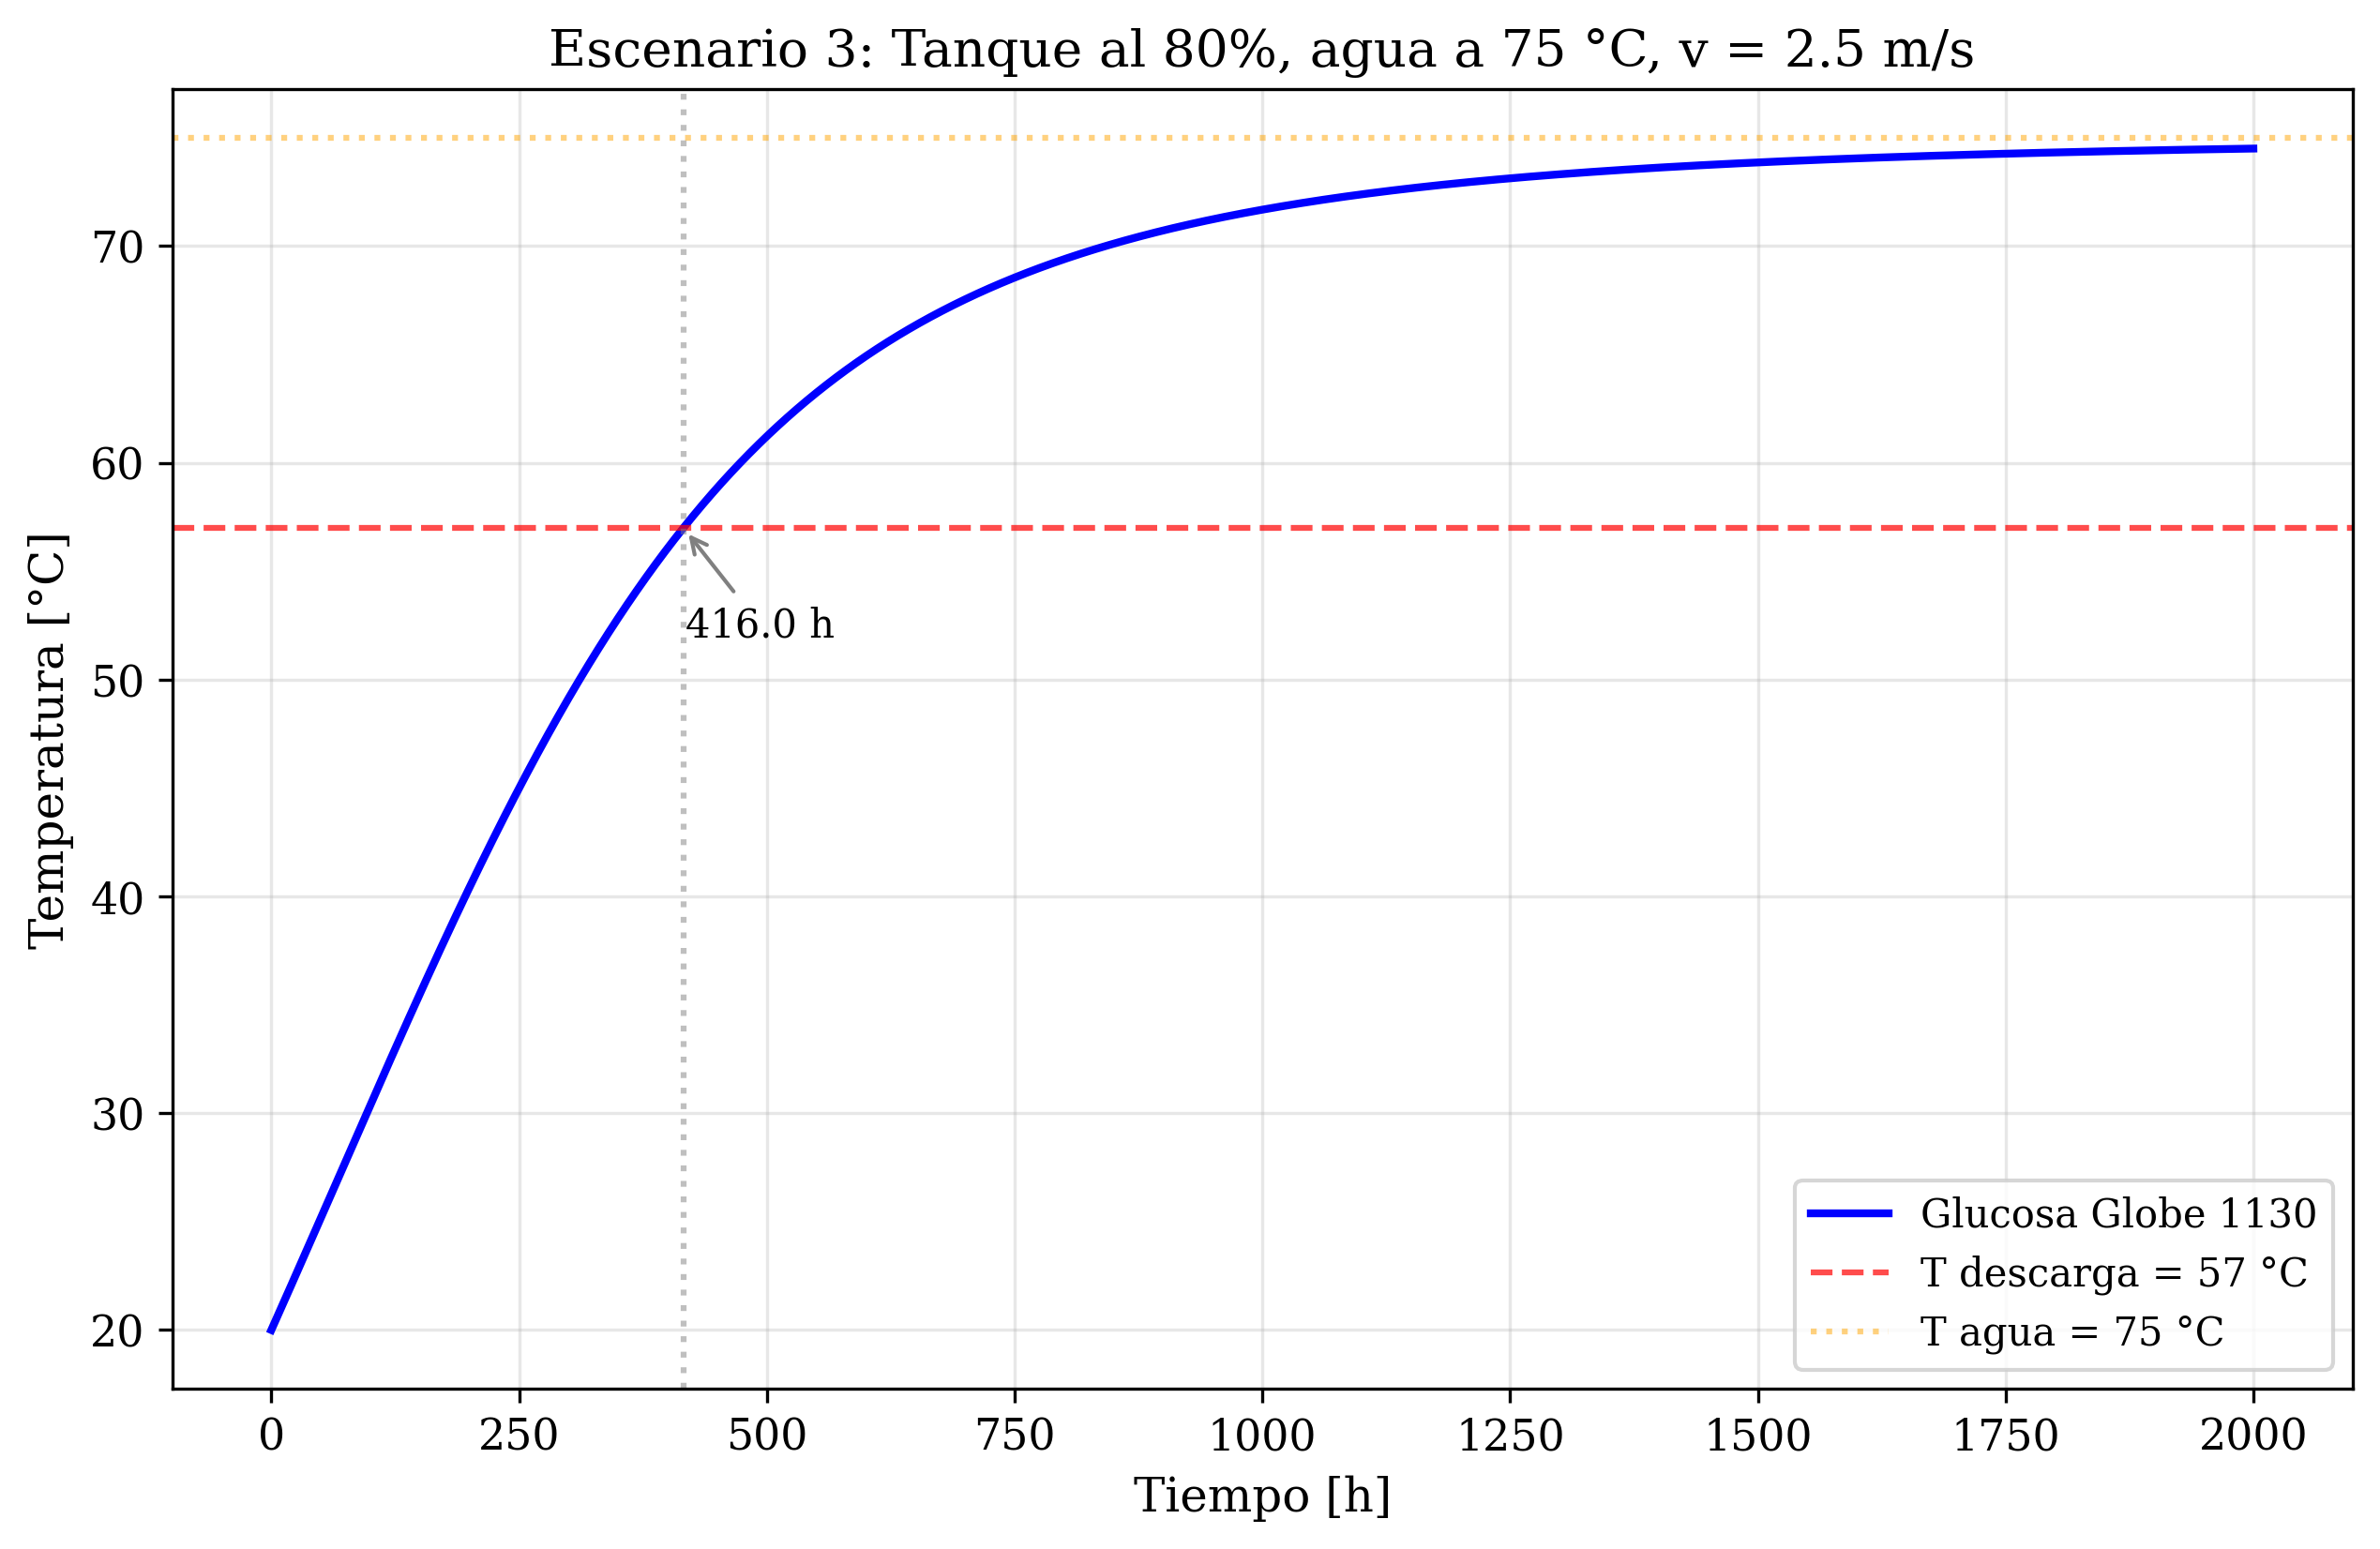
\includegraphics[width=0.85\textwidth]{../figures/escenario3_T_vs_tiempo.png}
	\caption{Escenario 3: Perfil de temperatura de la glucosa durante el calentamiento del tanque al 80\% ($T_{w,in}$ = 75~°C, $v_w$ = 2.5~m/s).}
	\label{fig:escenario3}
\end{figure}

\begin{figure}[H]
	\centering
	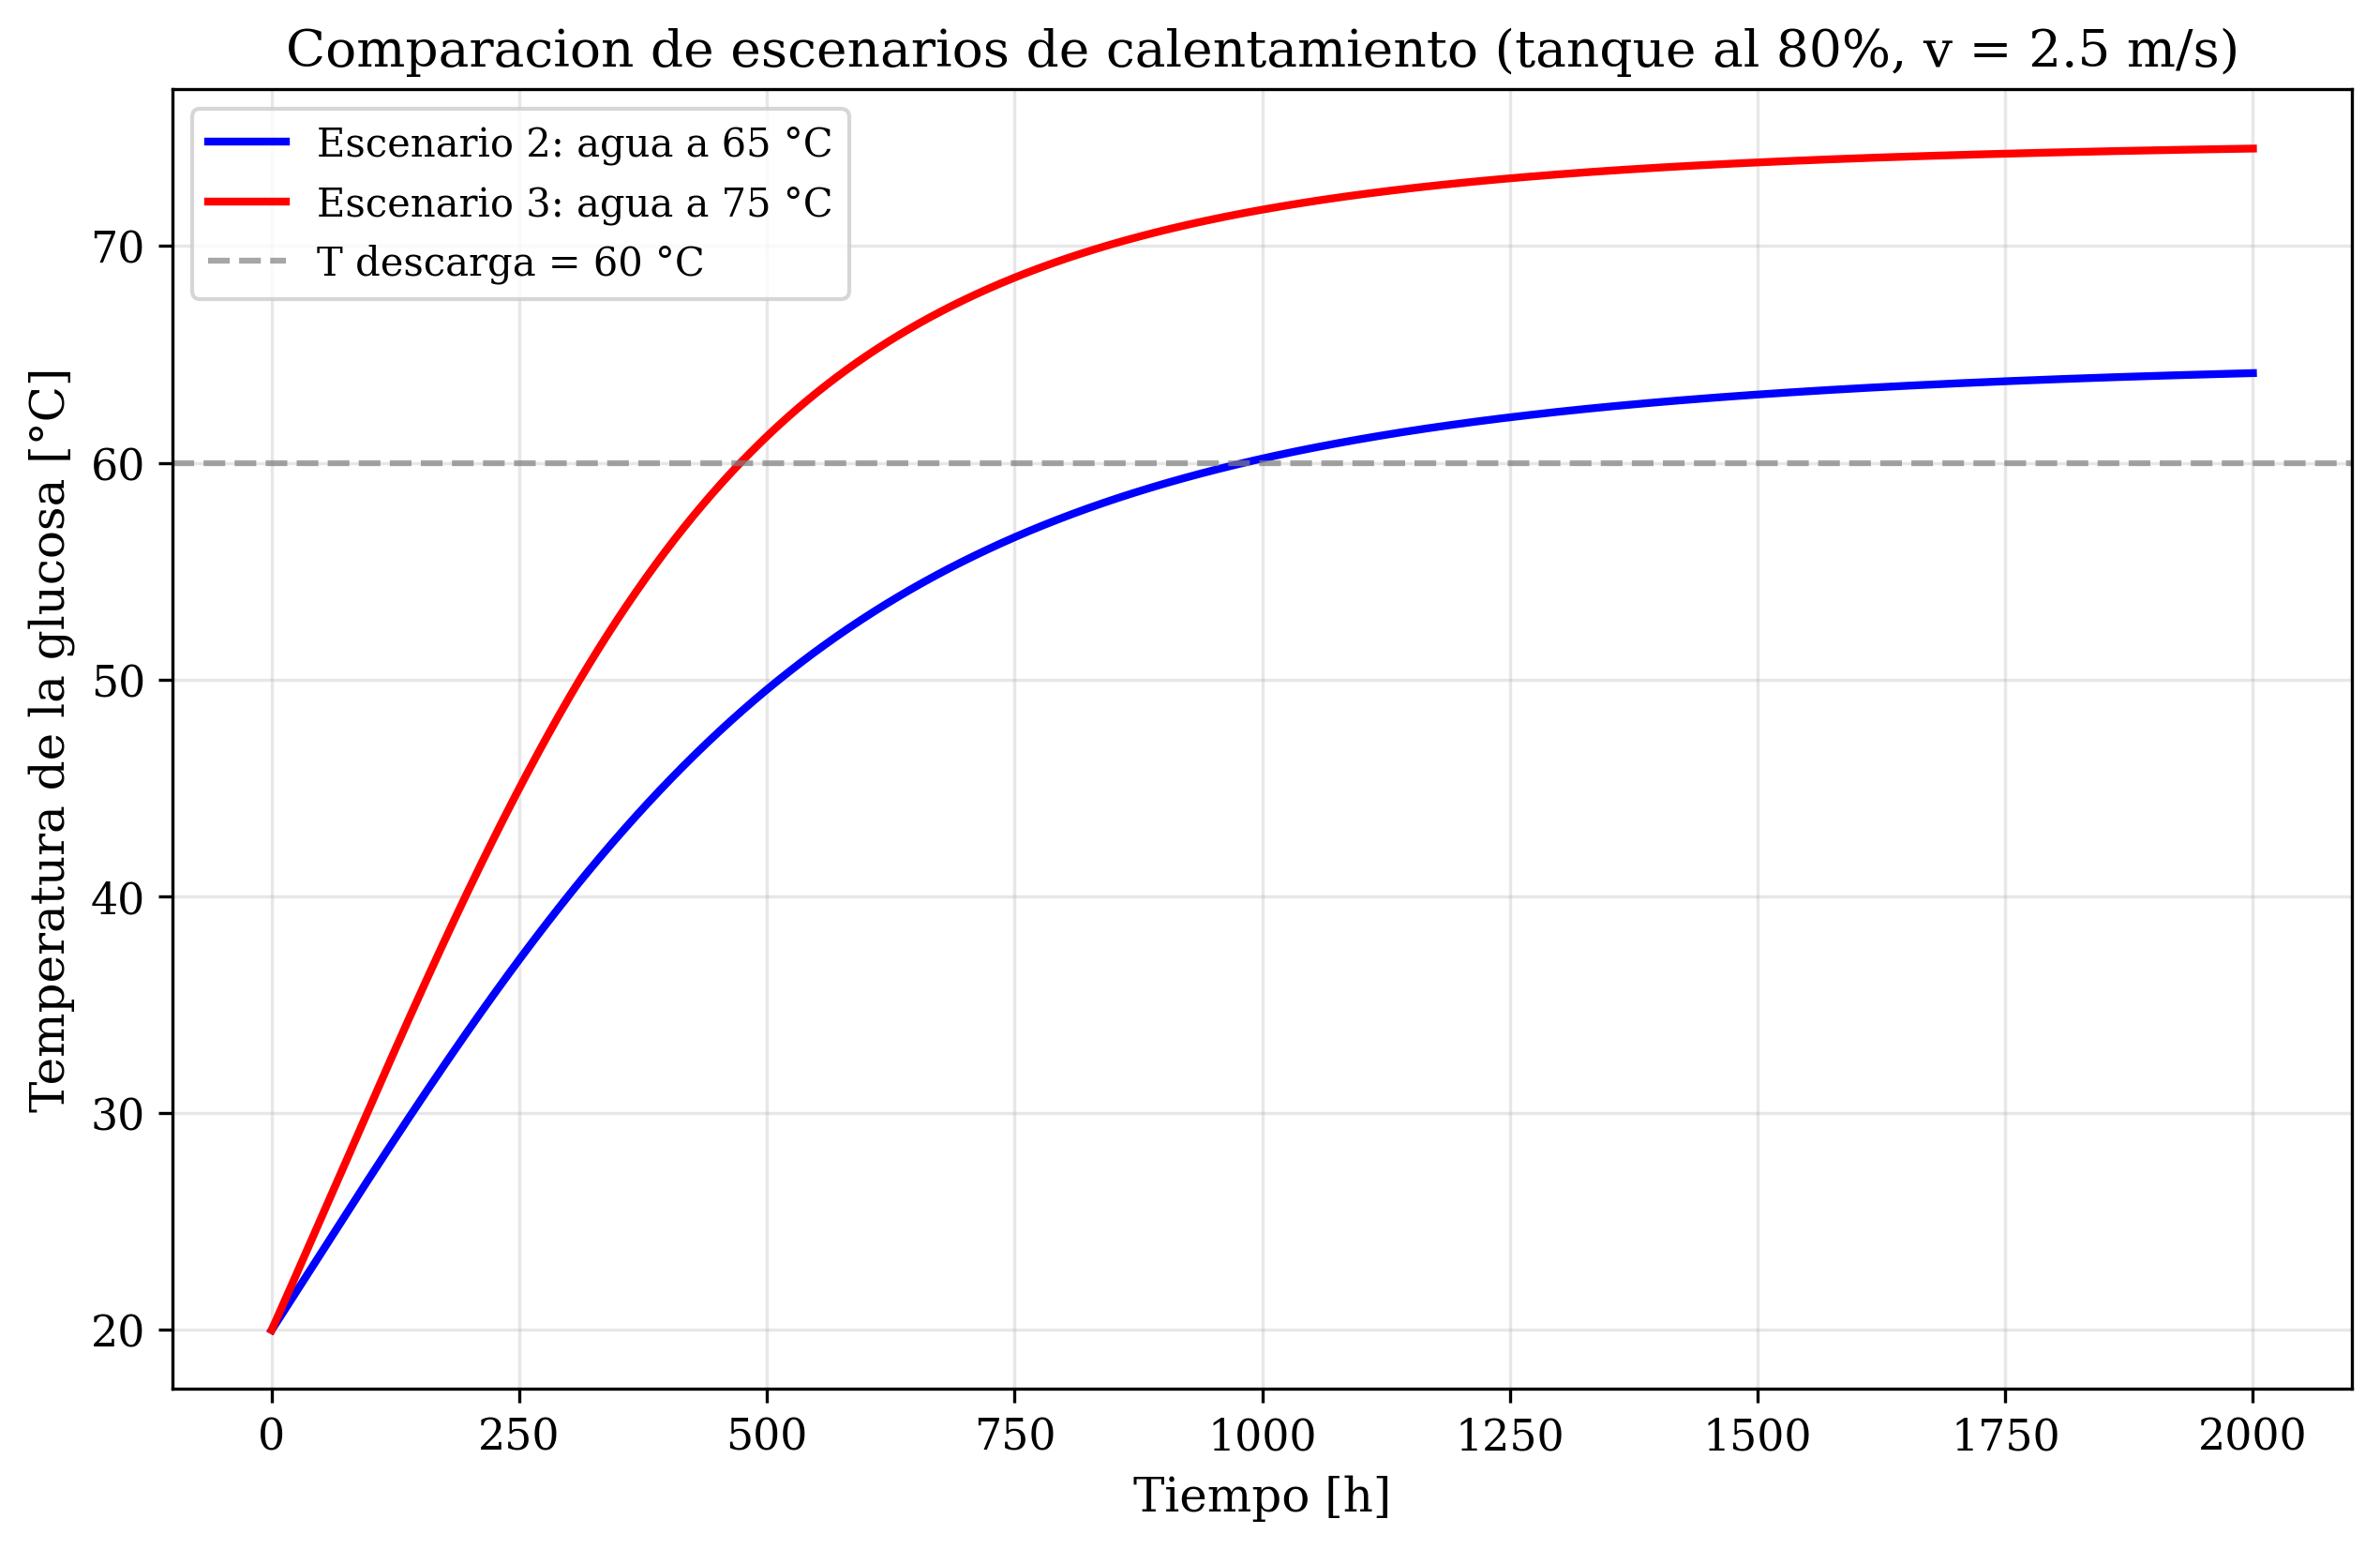
\includegraphics[width=0.85\textwidth]{../figures/comparacion_escenarios_2_3.png}
	\caption{Comparaci\'on de perfiles de temperatura para los Escenarios 2 ($T_w$ = 65~°C) y 3 ($T_w$ = 75~°C), tanque al 80\%, $v_w$ = 2.5~m/s.}
	\label{fig:comparacion}
\end{figure}

\subsubsection{Escenario 4: Ciclo Industrial de Despacho}

El Escenario~4 simula la operaci\'on industrial de despacho de 192~toneladas de glucosa (8~carrotanques de 24~toneladas cada uno), partiendo de una masa ya precalentada a 55~°C. La temperatura del agua de calentamiento es 75~°C y la temperatura m\'inima de despacho es 57~°C. El ciclo operativo consiste en recalentar la glucosa hasta 57~°C, descargar un carrotanque de 24~toneladas en 1.5~horas (mientras el calentamiento contin\'ua), y repetir este proceso 8~veces hasta el vaciado pr\'acticamente completo del tanque. La Tabla~\ref{tab:esc4_ciclo} resume los resultados por descarga.

\begin{table}[H]
	\centering
	\caption{Escenario 4: Ciclo de 8~descargas de 24~ton ($T_{w,in}$ = 75~°C, $T_{desc}$ = 57~°C, $v_w$ = 2.5~m/s).}
	\label{tab:esc4_ciclo}
	\setcounter{itemcount}{0}
	\begin{tabularx}{\textwidth}{@{}NcccccX@{}}
		\toprule
		\multicolumn{1}{c}{\textbf{Item}} & \textbf{Descarga} & \textbf{$\Delta t_{recal}$ [h]} & \textbf{$T_{ini}$ [°C]} & \textbf{$T_{fin}$ [°C]} & \textbf{$m_{ini}$ [ton]} & \textbf{$m_{fin}$ [ton]} \\
		\midrule
		& 1 & 25.5 & 57.0 & 57.1 & 192.0 & 168.0 \\
		& 2 & 0 & 57.1 & 57.3 & 168.0 & 144.0 \\
		& 3 & 0 & 57.3 & 57.4 & 144.0 & 120.0 \\
		& 4 & 0 & 57.4 & 57.6 & 120.0 & 96.0 \\
		& 5 & 0 & 57.6 & 57.9 & 96.0 & 72.0 \\
		& 6 & 0 & 57.9 & 58.2 & 72.0 & 48.0 \\
		& 7 & 0 & 58.2 & 58.8 & 48.0 & 24.0 \\
		& 8 & 0 & 58.8 & 60.0 & 24.0 & 0.5 \\
		\bottomrule
	\end{tabularx}
\end{table}

El resultado m\'as significativo del Escenario~4 es que \textbf{solo la primera descarga requiere un tiempo de recalentamiento}, de 25.5~horas (55~°C $\to$ 57~°C para 192~toneladas). Esta duraci\'on es consecuencia directa de la alt\'isima viscosidad de la glucosa a 55~°C ($\sim$4\,870~cP), que limita severamente la convecci\'on natural del lado del producto. A partir de la segunda descarga, la temperatura de la glucosa \textbf{nunca cae por debajo de 57~°C}, ejecut\'andose las 7~descargas restantes de forma consecutiva.

La temperatura de la glucosa se incrementa gradualmente a lo largo del ciclo desde 57.0~°C en la primera descarga hasta topar con la restricci\'on operativa recomendada m\'axima de \textbf{60.0~°C} en la \'ultima descarga. El tiempo total del ciclo completo log\'istico es de \textbf{37.5~horas}. Las Figuras~\ref{fig:esc4_ciclo_T} y \ref{fig:esc4_gantt} presentan los perfiles de temperatura y el diagrama de Gantt del ciclo.

\begin{figure}[H]
	\centering
	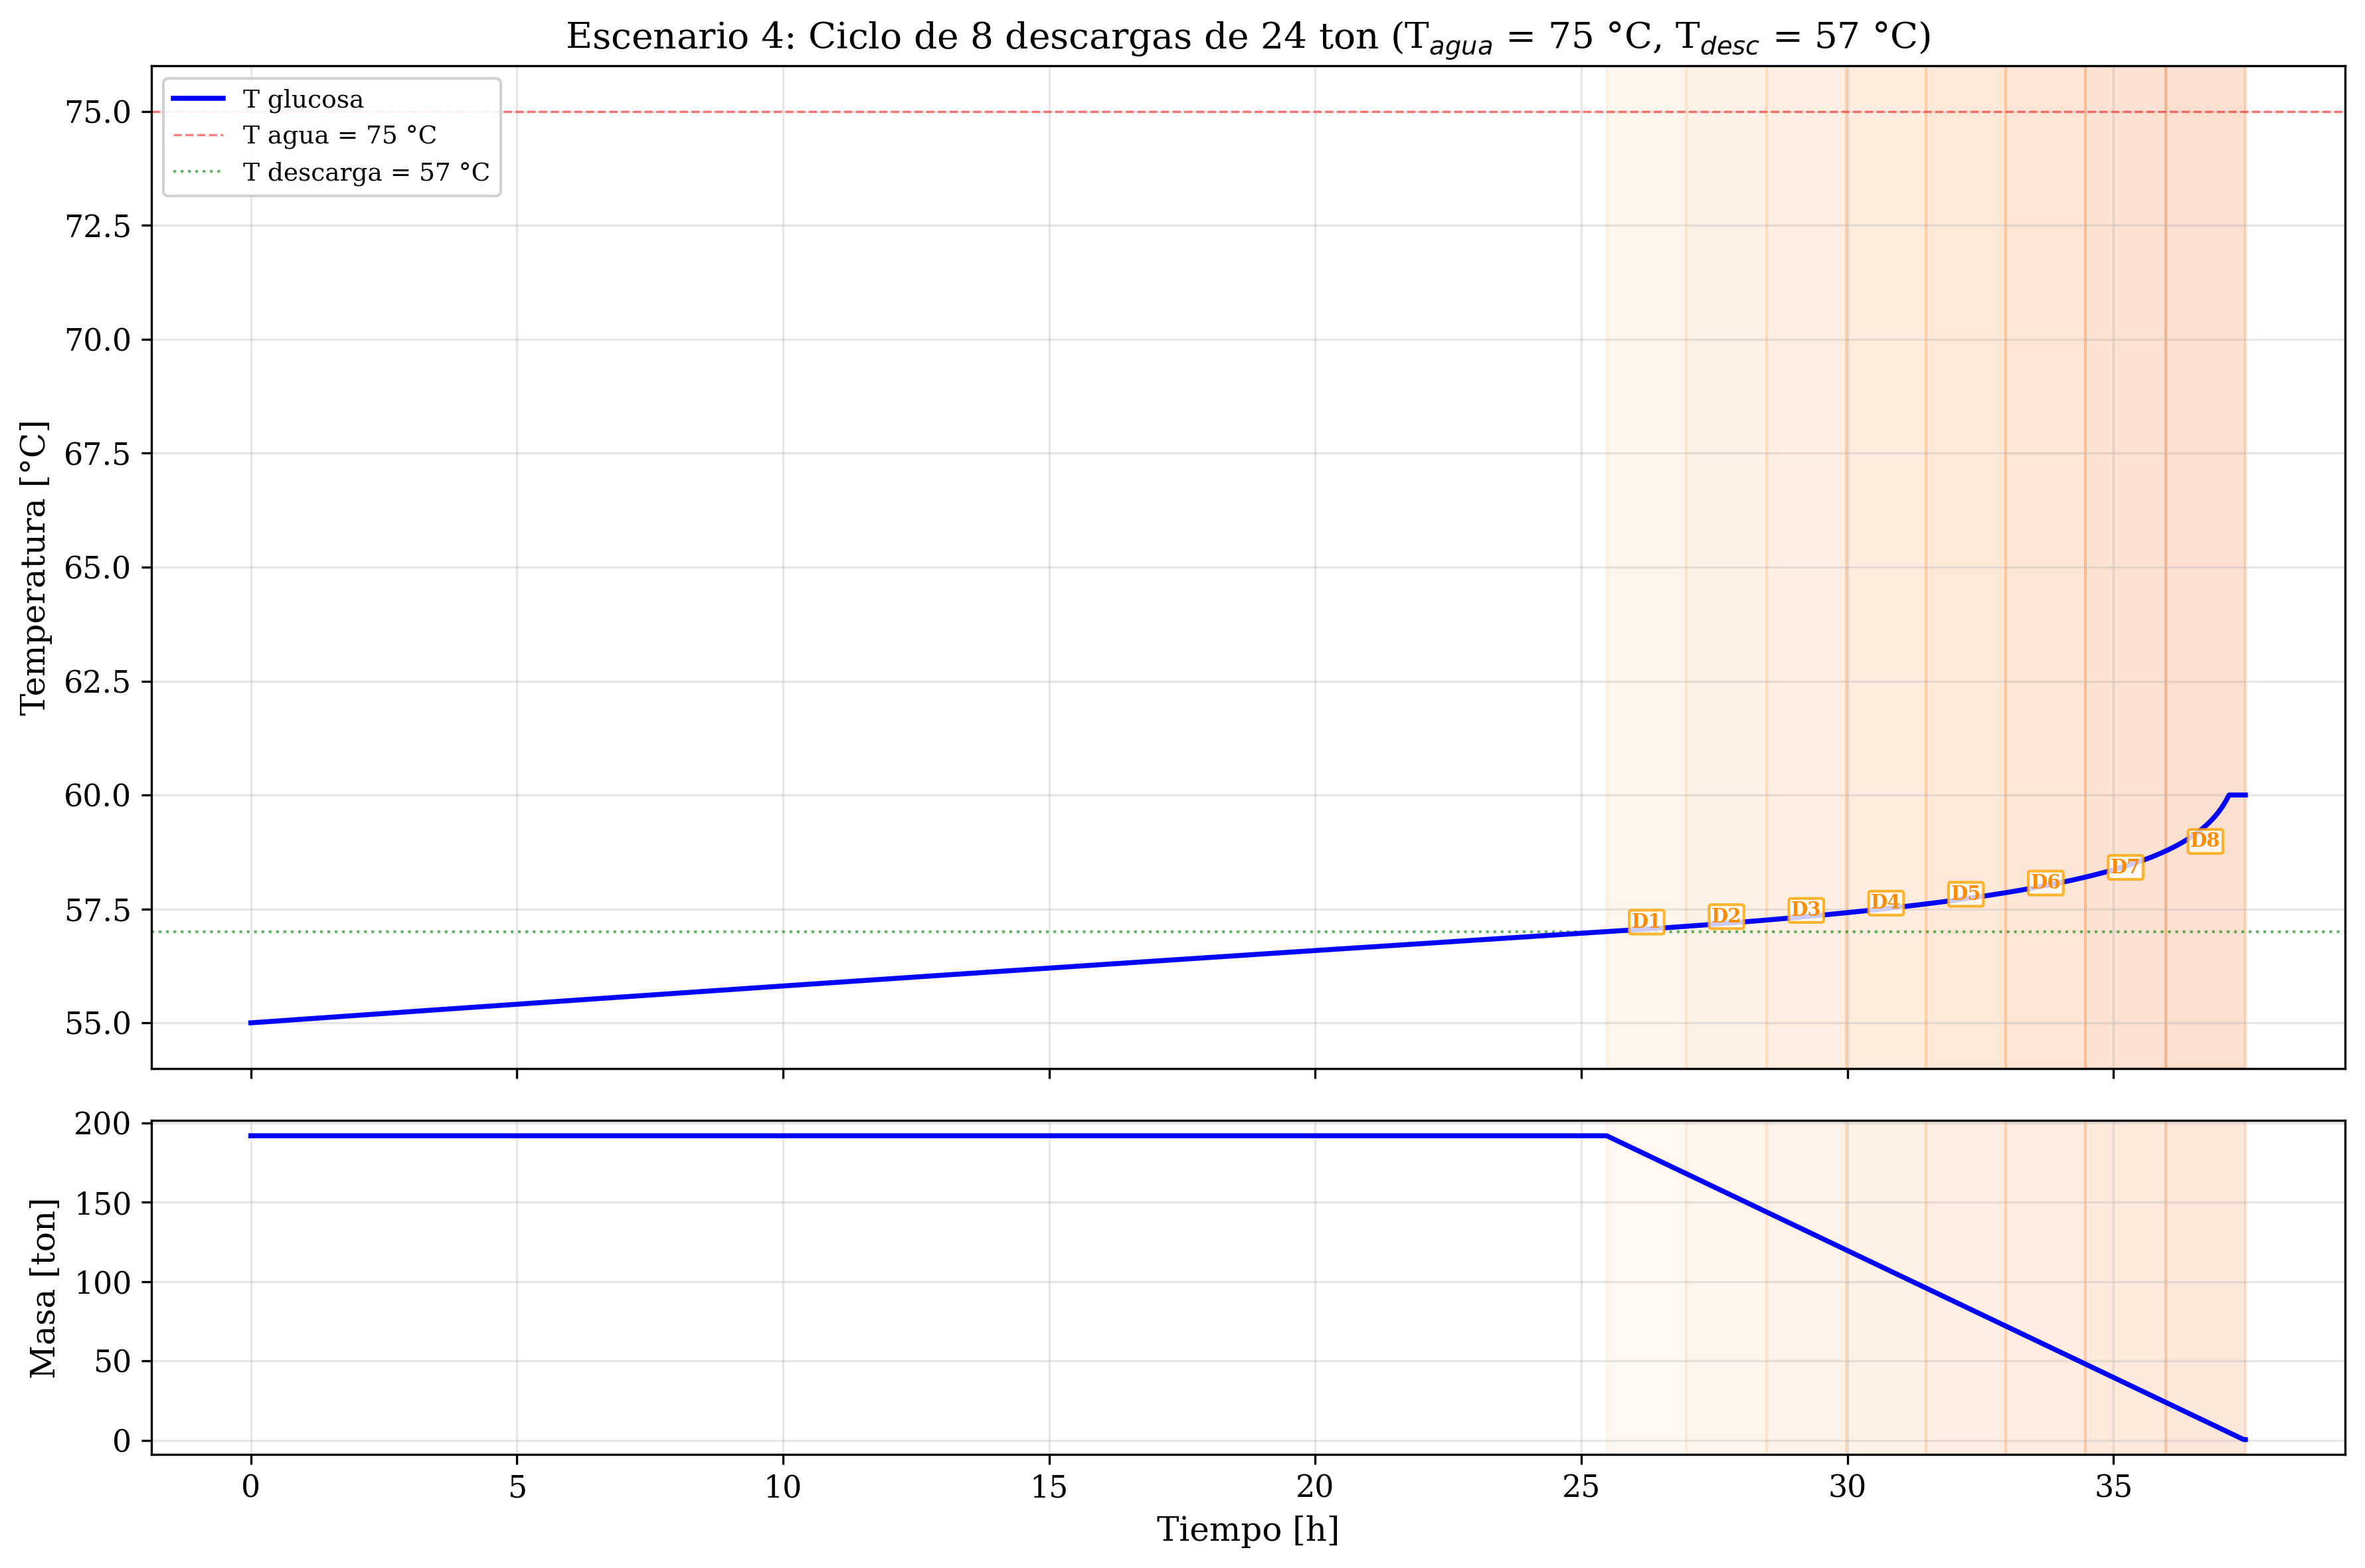
\includegraphics[width=0.95\textwidth]{../figures/escenario4_ciclo_T.png}
	\caption{Escenario 4: Perfil de temperatura (panel superior) y masa residual (panel inferior) durante el ciclo de 8 descargas de 24~ton. Las bandas sombreadas indican las fases de descarga as\'i como el topado protector recomendado.}
	\label{fig:esc4_ciclo_T}
\end{figure}

\begin{figure}[H]
	\centering
	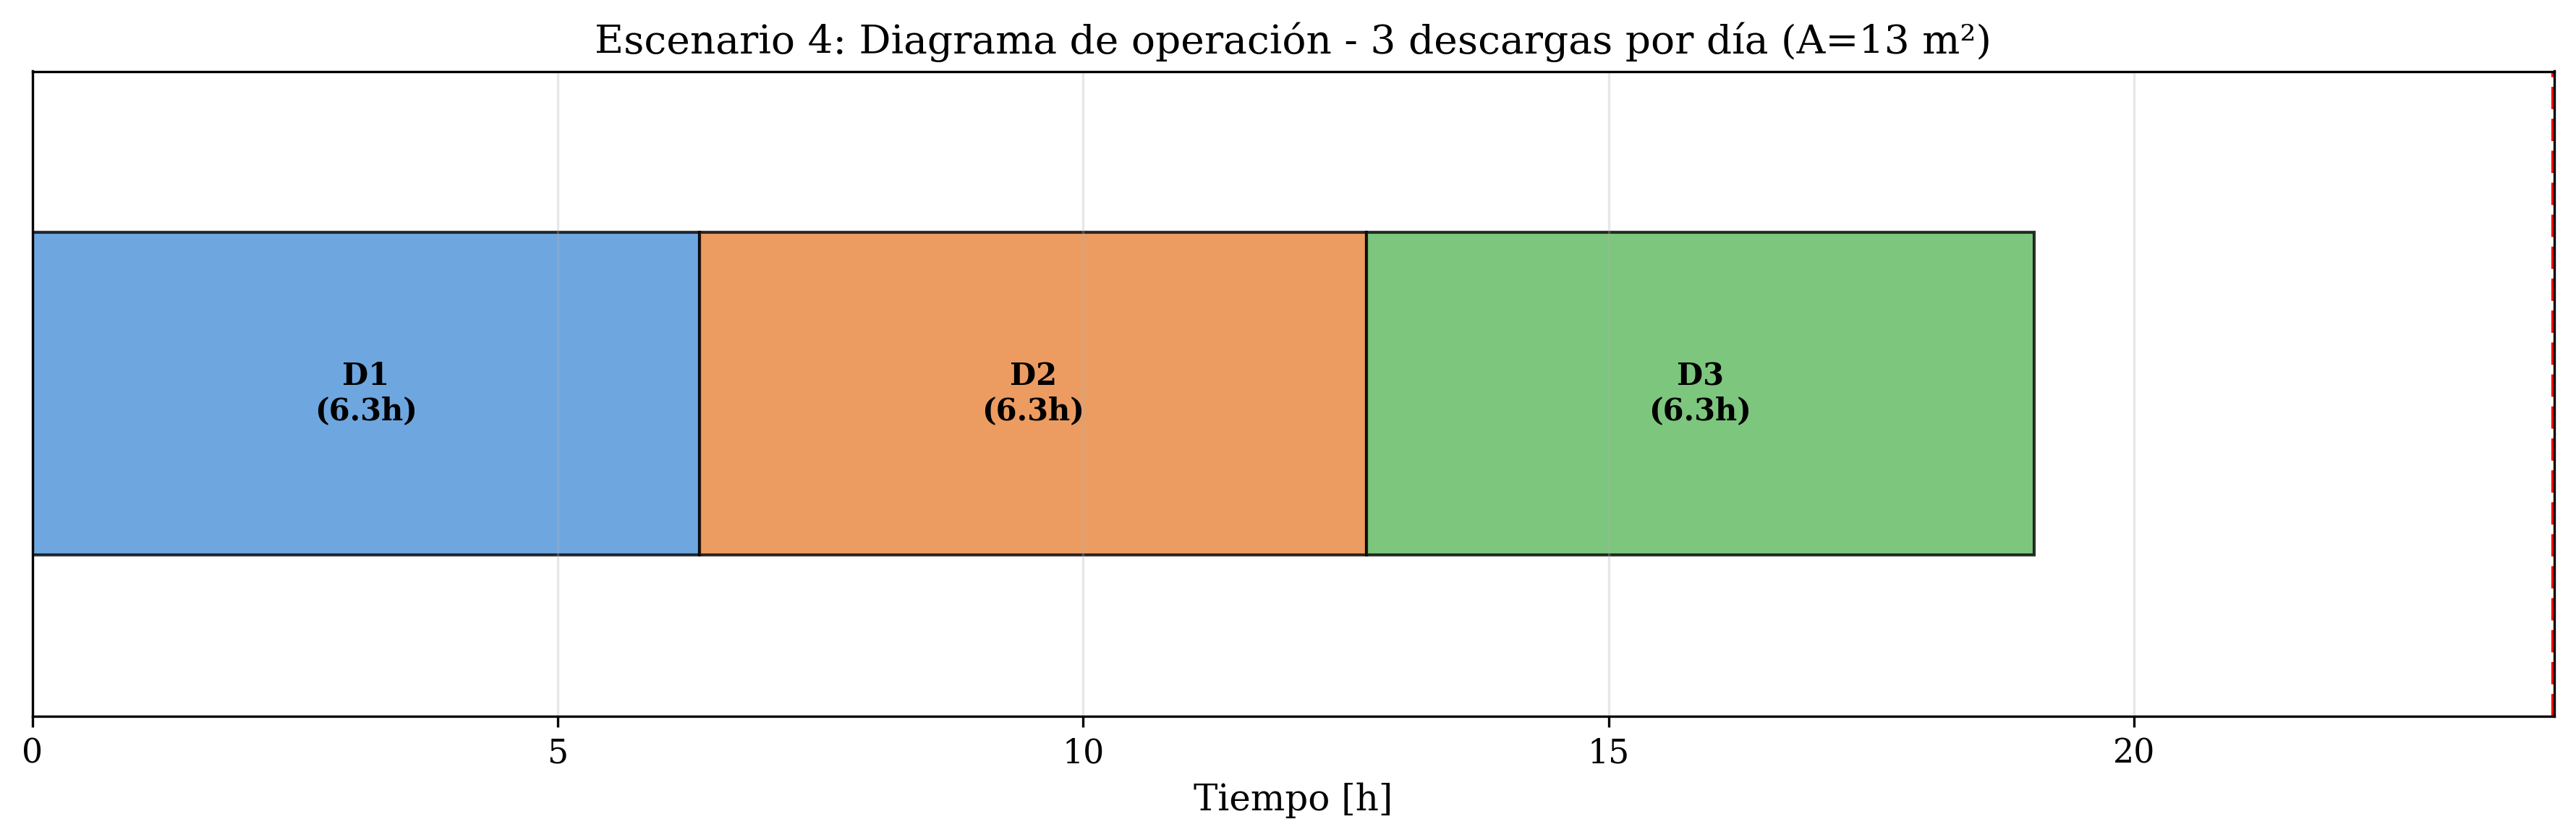
\includegraphics[width=0.95\textwidth]{../figures/escenario4_gantt.png}
	\caption{Diagrama de Gantt del Escenario~4: 25.5~h de recalentamiento inicial (azul) seguidas de 8 descargas consecutivas de 1.5~h (naranja). Tiempo total: 37.5~h.}
	\label{fig:esc4_gantt}
\end{figure}

\subsubsection{Ciclo de Descargas a Carrotanque --- Escenarios 2 y 3}

Para los Escenarios~2 y 3, se simul\'o el ciclo operativo de 8~descargas de 24~toneladas cada una, con un per\'iodo de 3~horas (1.5~h de descarga + 1.5~h de calentamiento entre descargas), para un tiempo total de 24~horas. La temperatura inicial del ciclo log\'istico es 57~°C (alcanzada tras el precalentamiento masivo). Las Tablas~\ref{tab:ciclo_esc2} y \ref{tab:ciclo_esc3} presentan los resultados con el condicionante de techo t\'ermico en los 60.0~°C.

\begin{table}[H]
	\centering
	\caption{Ciclo de 8 descargas de 24~ton -- Escenario 2 ($T_{w,in}$ = 65~°C, 24~h).}
	\label{tab:ciclo_esc2}
	\setcounter{itemcount}{0}
	\begin{tabularx}{\textwidth}{@{}NccccccX@{}}
		\toprule
		\multicolumn{1}{c}{\textbf{Item}} & \textbf{Desc.} & \textbf{$t_{ini}$ [h]} & \textbf{$T_{ini}$ [°C]} & \textbf{$T_{fin}$ [°C]} & \textbf{$m_{ini}$ [ton]} & \textbf{$m_{fin}$ [ton]} & \textbf{Obs.} \\
		\midrule
		& 1 & 0.0 & 57.00 & 57.15 & 249.8 & 225.8 & -- \\
		& 2 & 3.0 & 57.30 & 57.46 & 225.8 & 201.8 & -- \\
		& 3 & 6.0 & 57.62 & 57.79 & 201.8 & 177.8 & -- \\
		& 4 & 9.0 & 57.97 & 58.15 & 177.8 & 153.8 & -- \\
		& 5 & 12.0 & 58.34 & 58.54 & 153.8 & 129.8 & -- \\
		& 6 & 15.0 & 58.75 & 58.98 & 129.8 & 105.8 & -- \\
		& 7 & 18.0 & 59.22 & 59.47 & 105.8 & 81.8 & -- \\
		& 8 & 21.0 & 59.75 & 60.00 & 81.8 & 57.8 & Topea a $60.0^\circ\mathrm{C}$ limit.\\
		\bottomrule
	\end{tabularx}
\end{table}

\begin{table}[H]
	\centering
	\caption{Ciclo de 8 descargas de 24~ton -- Escenario 3 ($T_{w,in}$ = 75~°C, 24~h).}
	\label{tab:ciclo_esc3}
	\setcounter{itemcount}{0}
	\begin{tabularx}{\textwidth}{@{}NccccccX@{}}
		\toprule
		\multicolumn{1}{c}{\textbf{Item}} & \textbf{Desc.} & \textbf{$t_{ini}$ [h]} & \textbf{$T_{ini}$ [°C]} & \textbf{$T_{fin}$ [°C]} & \textbf{$m_{ini}$ [ton]} & \textbf{$m_{fin}$ [ton]} & \textbf{Obs.} \\
		\midrule
		& 1 & 0.0 & 57.00 & 57.45 & 249.8 & 225.8 & -- \\
		& 2 & 3.0 & 57.92 & 58.39 & 225.8 & 201.8 & -- \\
		& 3 & 6.0 & 58.89 & 59.39 & 201.8 & 177.8 & -- \\
		& 4 & 9.0 & 59.92 & 60.00 & 177.8 & 153.8 & Alcanza lim. superior \\
		& 5 & 12.0 & 60.00 & 60.00 & 153.8 & 129.8 & Termostato en off \\
		& 6 & 15.0 & 60.00 & 60.00 & 129.8 & 105.8 & Termostato en off \\
		& 7 & 18.0 & 60.00 & 60.00 & 105.8 & 81.8 & Termostato en off \\
		& 8 & 21.0 & 60.00 & 60.00 & 81.8 & 57.8 & Termostato en off \\
		\bottomrule
	\end{tabularx}
\end{table}

En el Escenario~2 (agua a 65~°C), la temperatura de la glucosa se mantiene en un rango estrecho durante gran parte del d\'ia, partiendo en 57.0~°C y logrando ascender a los 60.0~°C al final del total de las 24~horas del ciclo. En el Escenario~3 (agua a 75~°C), la temperatura se incrementa progresivamente y de forma acelerada por el elevado gradiente; permitiendo saturar el objetivo de control de los 60.0~°C a partir de la descaga 4, y luego es mantenida a raya el resto de despachos previniendo un colapso en el producto. Las Figuras~\ref{fig:ciclo_esc2}, \ref{fig:ciclo_esc3} y \ref{fig:ciclo_gantt} presentan los perfiles de temperatura l\'imites y el diagrama de Gantt comparativo.

\begin{figure}[H]
	\centering
	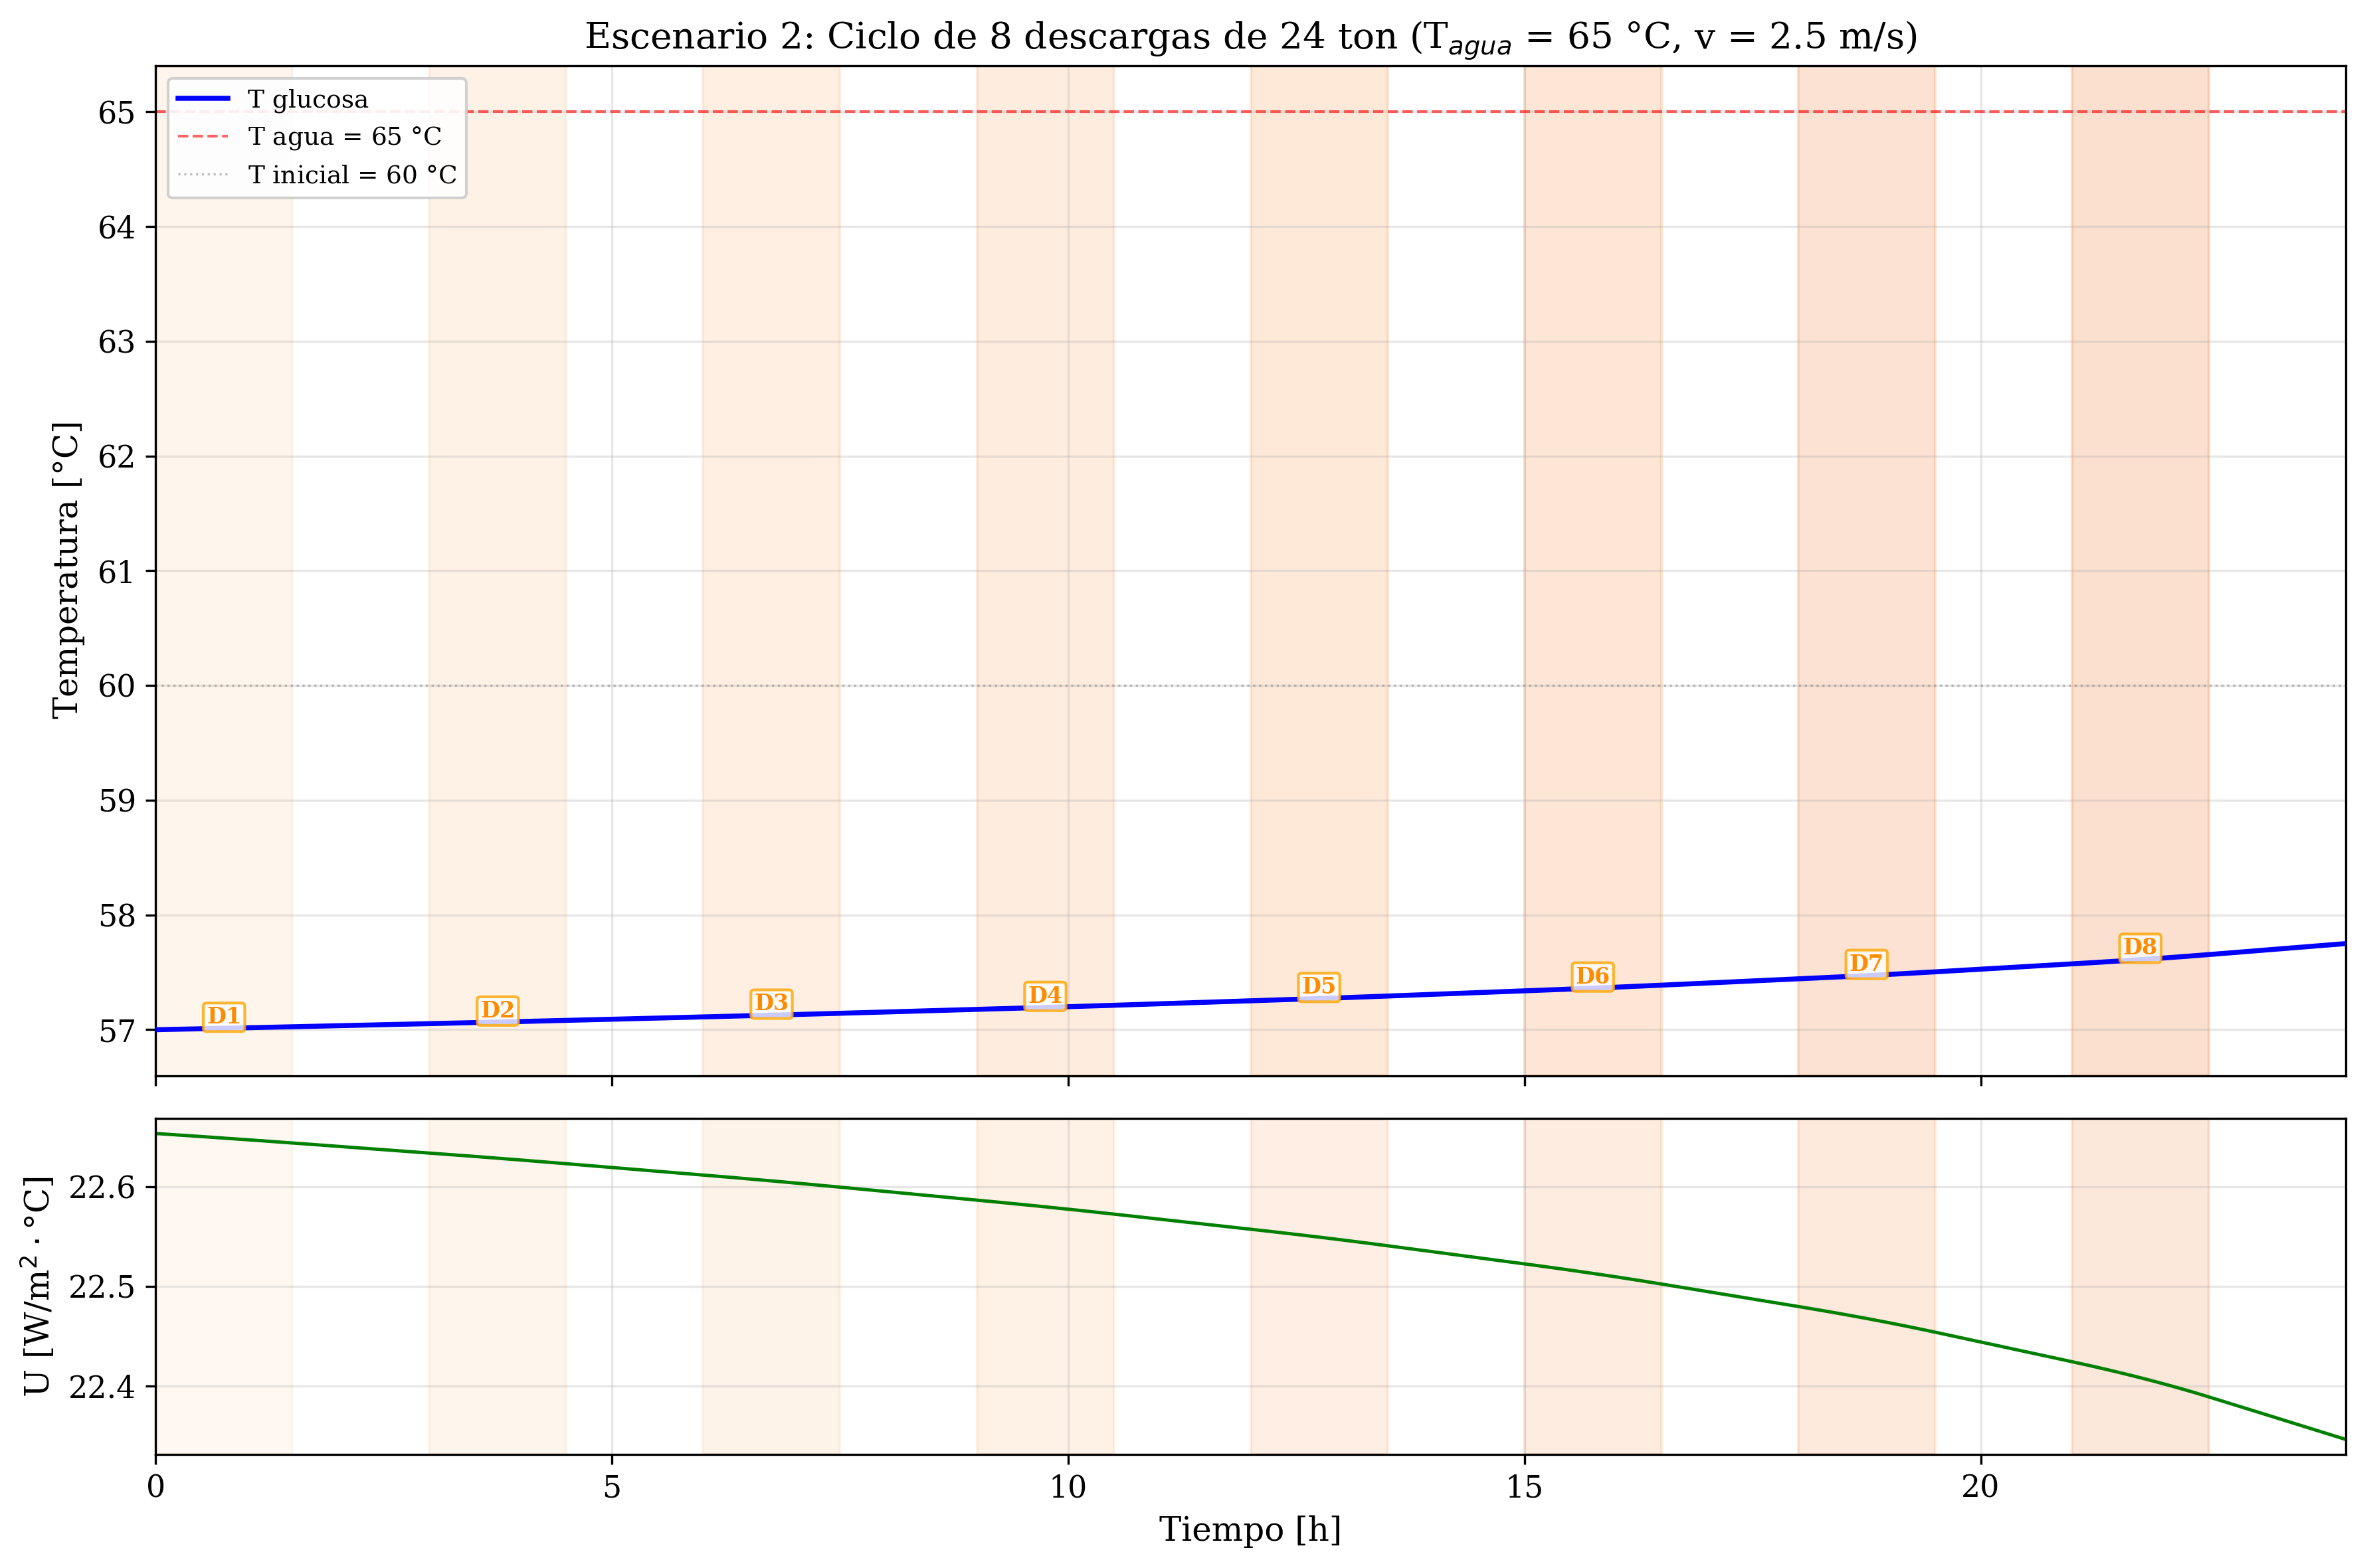
\includegraphics[width=0.85\textwidth]{../figures/ciclo_T_vs_tiempo_esc2.png}
	\caption{Ciclo de 8 descargas (Escenario~2): Temperatura y masa de glucosa durante 24~h ($T_{w,in}$ = 65~°C).}
	\label{fig:ciclo_esc2}
\end{figure}

\begin{figure}[H]
	\centering
	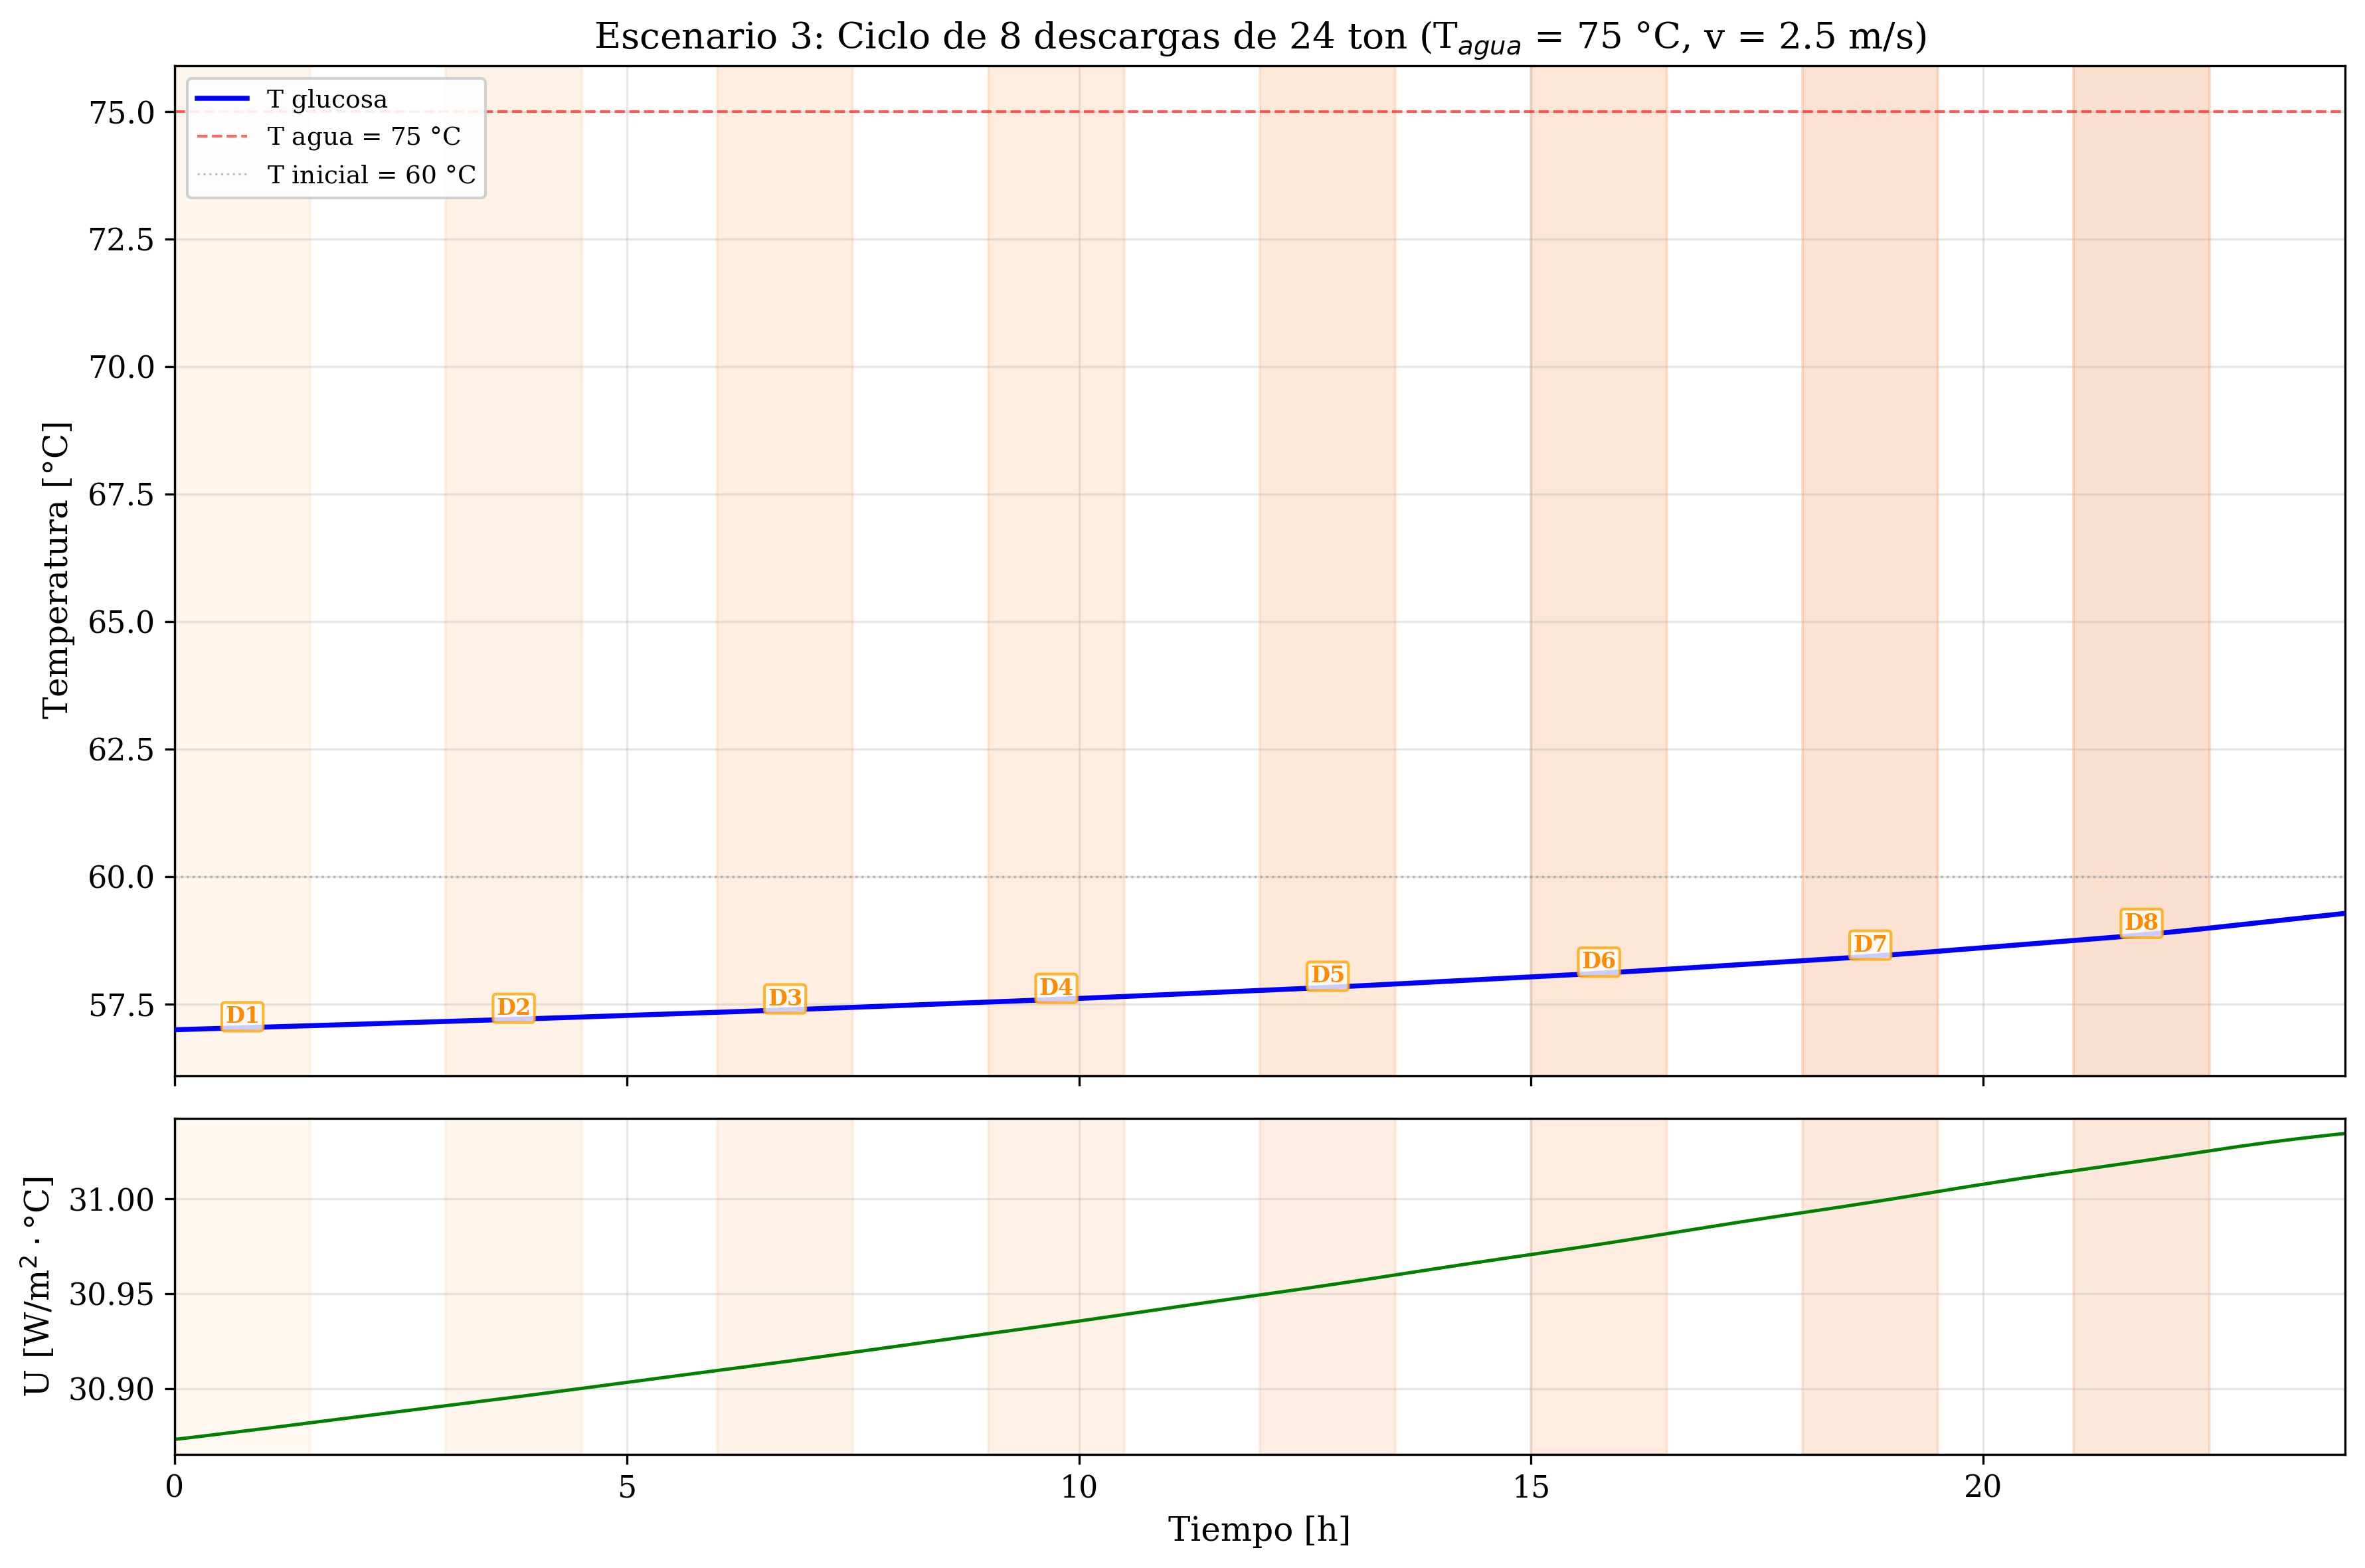
\includegraphics[width=0.85\textwidth]{../figures/ciclo_T_vs_tiempo_esc3.png}
	\caption{Ciclo de 8 descargas (Escenario~3): Temperatura y masa de glucosa durante 24~h ($T_{w,in}$ = 75~°C).}
	\label{fig:ciclo_esc3}
\end{figure}

\begin{figure}[H]
	\centering
	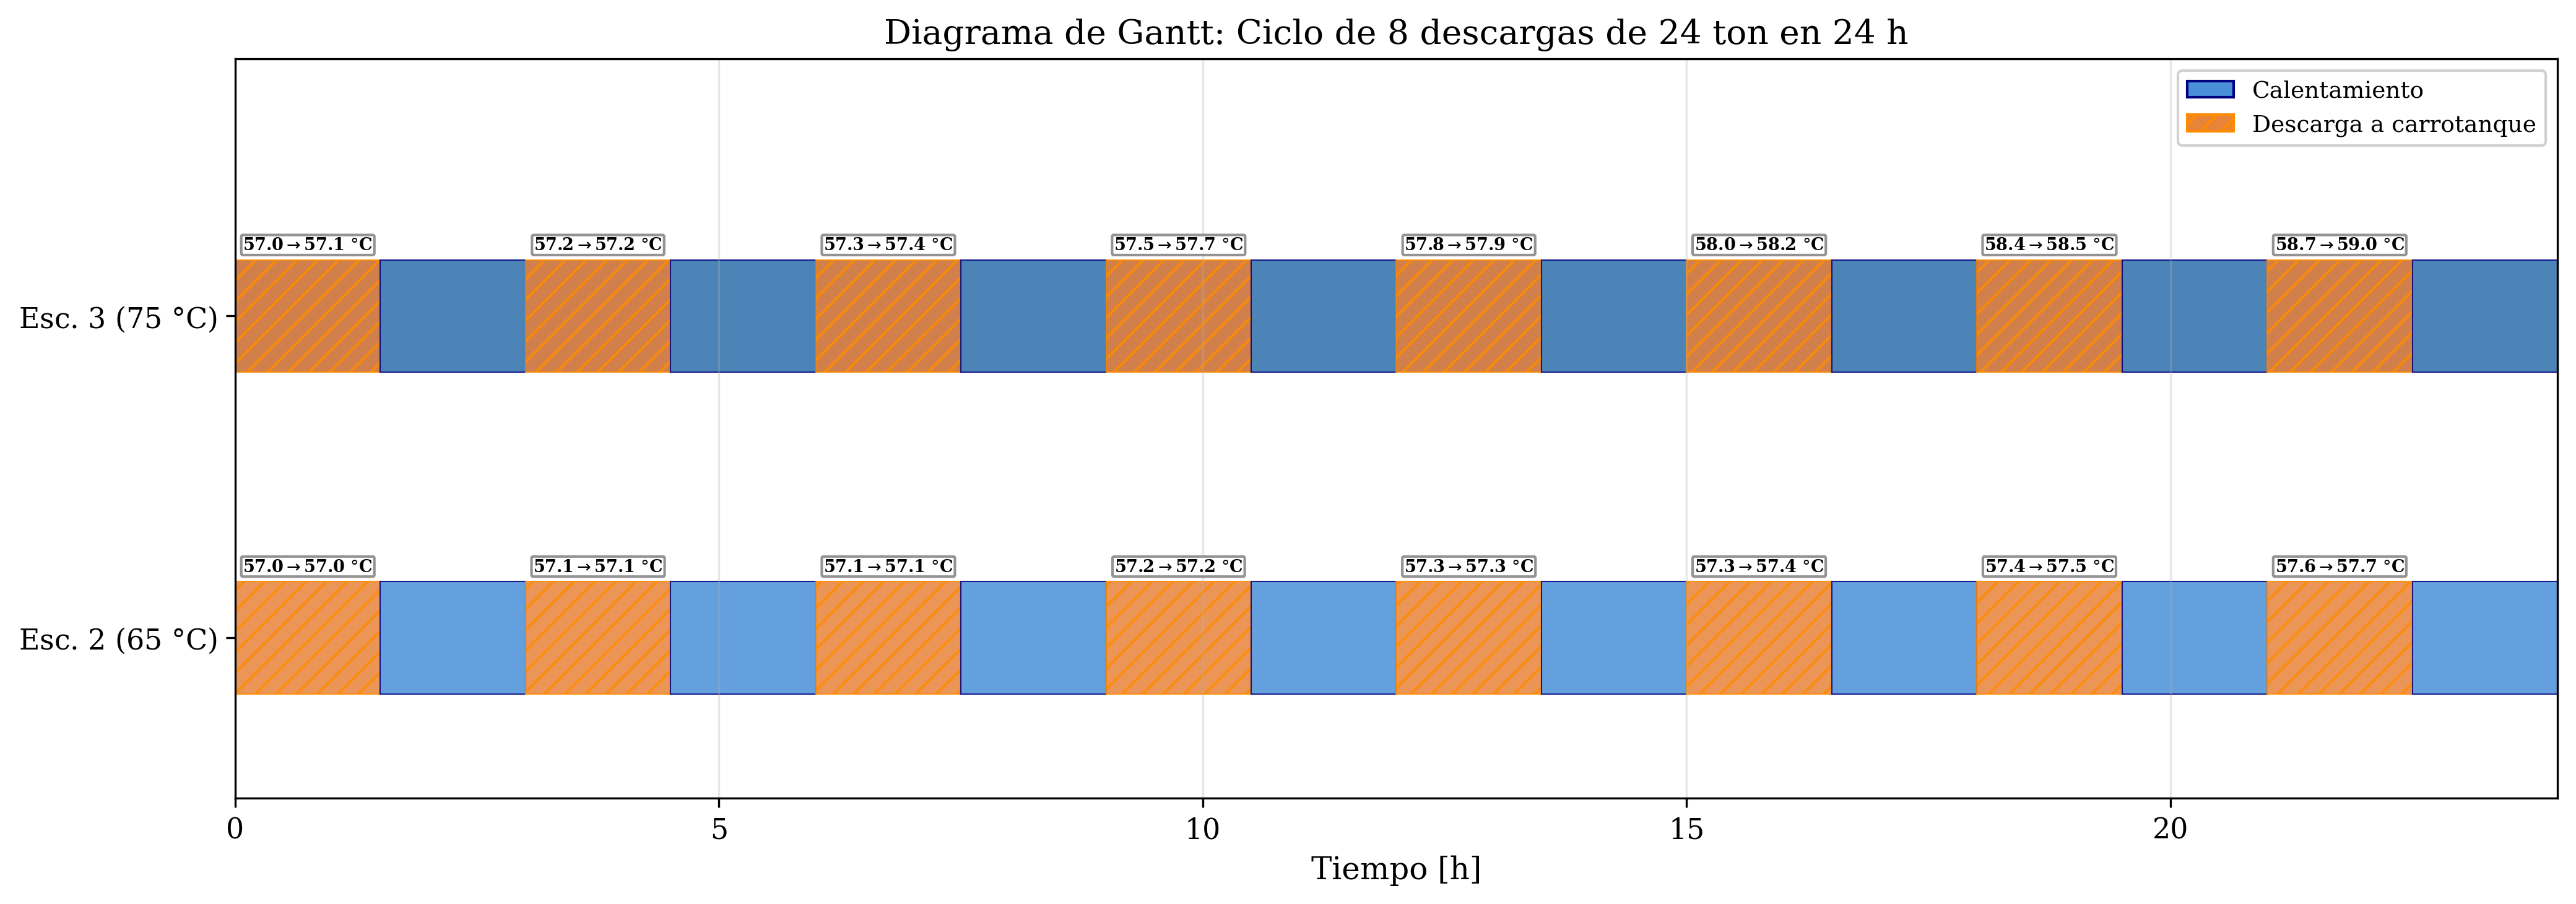
\includegraphics[width=0.95\textwidth]{../figures/ciclo_gantt.png}
	\caption{Diagrama de Gantt comparativo del ciclo de 8~descargas para los Escenarios~2 y 3.}
	\label{fig:ciclo_gantt}
\end{figure}

\subsubsection{Espesor de Aislamiento T\'ermico}

Se evalu\'o el efecto del espesor de aislamiento de lana mineral sobre las p\'erdidas de calor al ambiente y la temperatura superficial exterior de la chaqueta. La Tabla~\ref{tab:aislamiento} presenta los resultados para agua a 75\,°C (Escenario~3).

\begin{table}[H]
	\centering
	\caption{Efecto del espesor de aislamiento sobre p\'erdidas t\'ermicas y temperatura superficial ($T_w = 75$\,°C, $T_{amb} = 26.5$\,°C).}
	\label{tab:aislamiento}
	\setcounter{itemcount}{0}
	\begin{tabularx}{\textwidth}{@{}NccccX@{}}
		\toprule
		\multicolumn{1}{c}{\textbf{Item}} & \textbf{Espesor [mm]} & \textbf{$Q_{p\'erd}$ [kW]} & \textbf{$T_{sup}$ [°C]} & \textbf{Reducci\'on [\%]} & \textbf{Seguridad} \\
		\midrule
		& 0 (sin aislamiento) & 8.27 & 74.8 & 0 & No cumple \\
		& 12.7 (1/2'') & 2.34 & 40.2 & 71.7 & Cumple \\
		& 25.4 (1'') & 1.36 & 34.5 & 83.5 & Cumple \\
		& 38.1 (1.5'') & 0.96 & 32.1 & 88.4 & Cumple \\
		& \textbf{50.8 (2'')} & \textbf{0.74} & \textbf{30.8} & \textbf{91.0} & \textbf{Cumple} \\
		& 76.2 (3'') & 0.51 & 29.5 & 93.8 & Cumple \\
		\bottomrule
	\end{tabularx}
\end{table}

Sin aislamiento, la temperatura superficial alcanza 74.8\,°C (insegura al contacto) y las p\'erdidas al ambiente ascienden a 8.27~kW, lo que reduce la eficiencia del sistema de calentamiento. Con el espesor de dise\~no calculado y recomendado en este estudio (2'', 50.8~mm), la temperatura superficial desciende a 30.8\,°C (segura al contacto) y las p\'erdidas se reducen en un 91\%, a tan solo 0.74~kW. Este espesor constituye un punto de equilibrio adecuado entre eficiencia energ\'etica e inversi\'on: espesores superiores ofrecen mejoras marginales (de 91\% a 94\% con 3''), mientras que espesores inferiores como 1'' (25.4~mm) reducen las p\'erdidas un 83.5\%, lo que representa un 7.5\% menos de eficiencia. Se recomienda instalar lana mineral de 2'' (50.8~mm) sobre la chaqueta de media ca\~na como espesor t\'ecnicamente apropiado para esta aplicaci\'on.

\subsection{Validaci\'on Mediante Simulaci\'on CFD --- COMSOL Multiphysics~6.4}

La simulaci\'on de Din\'amica de Fluidos Computacional (CFD) del sistema de calentamiento se realiz\'o en COMSOL Multiphysics~6.4, bajo las condiciones del Escenario~3: glucosa Globe~42~DE a temperatura inicial de 25\,°C, agua caliente ingresando a la chaqueta de media ca\~na a 75\,°C con velocidad de 2.5\,m/s en el canal rectangular. La simulaci\'on model\'o el r\'egimen transitorio acoplado entre el flujo de agua en la espiral y la convecci\'on natural de la glucosa en el fondo toriesf\'erico, capturando la evoluci\'on espacial y temporal del campo de temperaturas desde el estado inicial hasta la estabilizaci\'on del sistema.

La Figura~\ref{fig:cfd1} presenta el campo de temperaturas obtenido para la condici\'on de arranque del sistema. La escala crom\'atica var\'ia entre 25\,°C (azul/violeta) y 75\,°C (rojo/naranja), revelando con precisi\'on la distribuci\'on t\'ermica tridimensional en el fondo toriesf\'erico y la chaqueta en espiral. En las espiras interiores, pr\'oximas al punto de entrada del agua, el fluido caliente mantiene temperaturas de 65 a 75\,°C (tonos naranja y amarillo), resultado de la cercan\'ia al suministro y del corto recorrido hidr\'aulico acumulado. A medida que el agua avanza a lo largo de la espiral hacia la periferia, la escala crom\'atica transita hacia verdes, cianes y azules, evidenciando el descenso progresivo de temperatura del fluido caliente conforme cede calor a la glucosa adyacente. El domo de glucosa aparece en azul y violeta, todav\'ia pr\'oximo a su temperatura inicial de 25\,°C, reflejo de la formidable inercia t\'ermica del jarabe ($\mu \approx 212\,000$\,cP a esa temperatura) y de su correspondiente resistencia a la convecci\'on natural.

\begin{figure}[H]
	\centering
	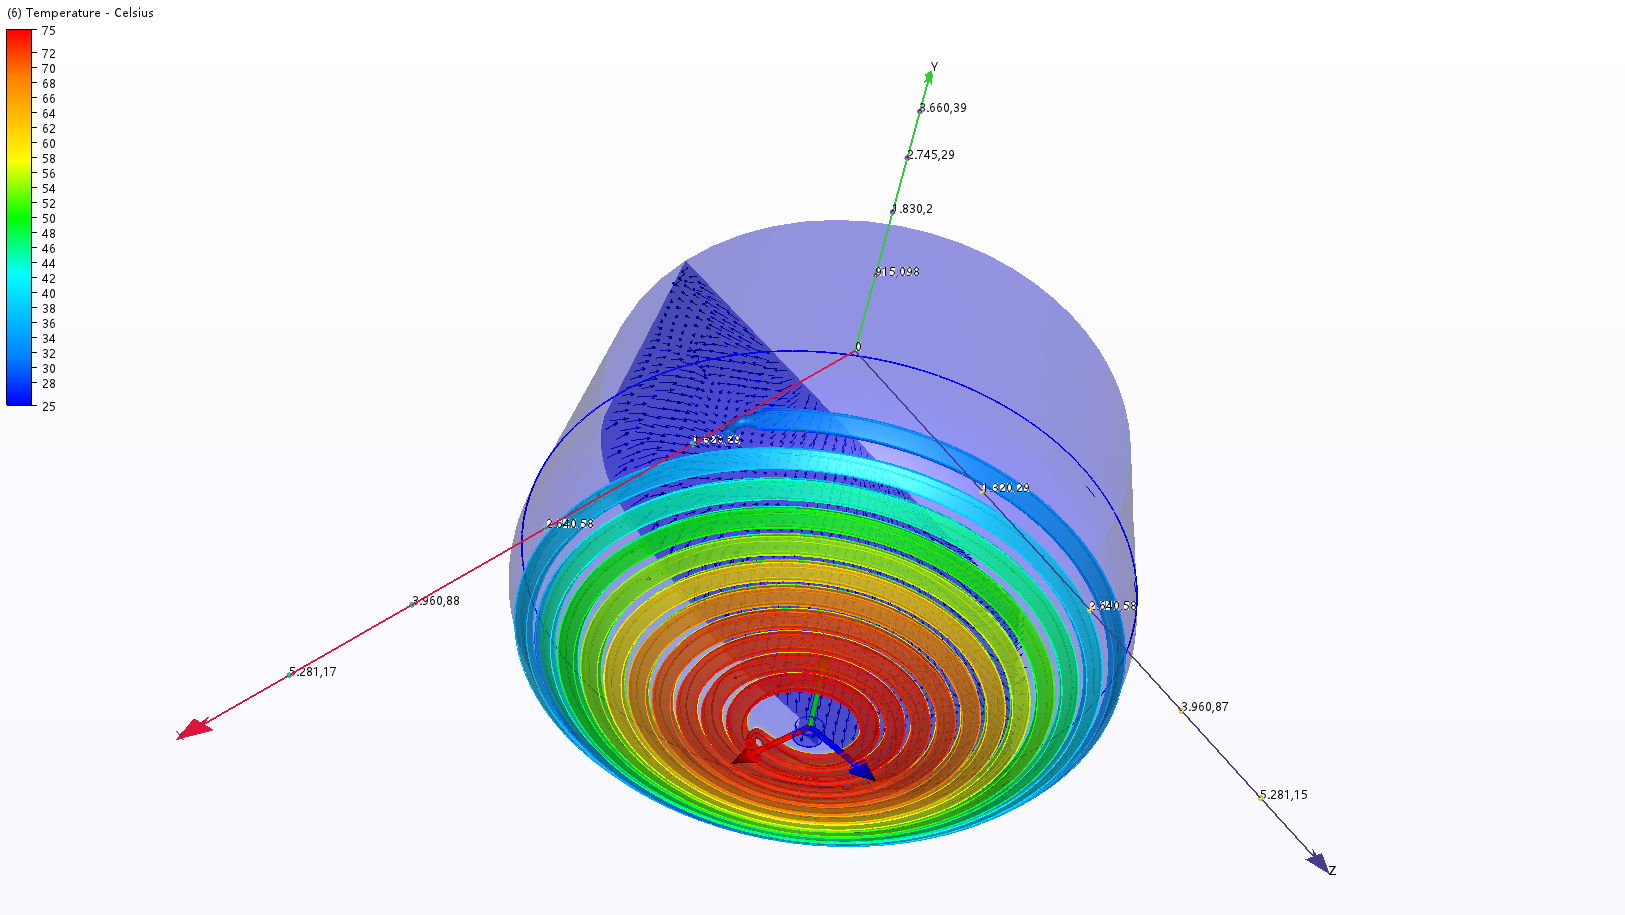
\includegraphics[width=0.85\textwidth]{../figures/cfd1.png}
	\caption{Campo de temperaturas (\textdegree C) en el fondo toriesf\'erico y la chaqueta de media ca\~na en espiral, obtenido mediante simulaci\'on CFD en COMSOL Multiphysics~6.4 (Escenario~3: $T_{g,0}=25$\,°C, $T_w=75$\,°C, $v_w=2.5$\,m/s). La transici\'on crom\'atica de naranja/amarillo en las espiras interiores (alta temperatura del agua entrante) hacia azul/violeta en las espiras exteriores y el volumen de glucosa ilustra el enfriamiento progresivo del fluido caliente a lo largo de la espiral y la elevada resistencia t\'ermica de la glucosa fr\'ia en el arranque.}
	\label{fig:cfd1}
\end{figure}

Este comportamiento en el arranque explica el bajo coeficiente de transferencia de calor registrado en los instantes iniciales de la simulaci\'on ($U_{\text{arranque}} \approx 10$\,W/m\textsuperscript{2}$\cdot$°C), dominado por la resistencia convectiva de la glucosa fr\'ia a 25\,°C. A medida que el jarabe se calienta progresivamente, su viscosidad disminuye de acuerdo con el modelo VFT calibrado a la ficha t\'ecnica Ingredion~011420, la convecci\'on natural mejora y el coeficiente global asciende hasta alcanzar un rango estable de 35 a 40\,W/m\textsuperscript{2}$\cdot$°C cuando el sistema opera en condiciones cuasi-estacionarias. La Tabla~\ref{tab:cfd_U} resume la comparaci\'on entre los coeficientes globales obtenidos por el modelo anal\'itico y la simulaci\'on CFD.

\begin{table}[H]
	\centering
	\caption{Comparaci\'on del coeficiente global de transferencia de calor $U$ entre el modelo anal\'itico y la simulaci\'on CFD (Escenario~3, $T_w=75$\,°C, $v_w=2.5$\,m/s).}
	\label{tab:cfd_U}
	\setcounter{itemcount}{0}
	\begin{tabularx}{\textwidth}{@{}NXcc@{}}
		\toprule
		\multicolumn{1}{c}{\textbf{Item}} & \textbf{Condici\'on / M\'etodo} & \textbf{$U$ [W/m\textsuperscript{2}$\cdot$°C]} & \textbf{Observaci\'on} \\
		\midrule
		& Anal\'itico --- arranque ($T_g = 25$\,°C) & $\approx 10$ & Viscosidad extrema: $\approx\!212\,000$\,cP \\
		& Anal\'itico --- estado estable ($T_g = 40$--$60$\,°C) & 26--36 & Convecci\'on natural mejorada \\
		& CFD (COMSOL~6.4) --- estado estable & \textbf{40.2} & Promedio ponderado sobre $A=13$\,m\textsuperscript{2} \\
		& Diferencia anal\'itico vs.\ CFD (estado estable) & +11\,\% & Concordancia satisfactoria \\
		\bottomrule
	\end{tabularx}
\end{table}

El coeficiente global promedio determinado por la simulaci\'on CFD en estado estable es $U_{\text{CFD}} = 40.2$\,W/m\textsuperscript{2}$\cdot$°C, valor que supera en un 11\,\% al resultado anal\'itico para la condici\'on m\'as cercana en temperatura ($U_{\text{anal\'itico}} = 36.2$\,W/m\textsuperscript{2}$\cdot$°C a $T_g = 60$\,°C). Esta concordancia es plenamente satisfactoria para ingenier\'ia de proceso, considerando que el modelo anal\'itico emplea correlaciones de convecci\'on natural desarrolladas para geometr\'ias ideales planas, mientras que la simulaci\'on CFD captura la geometr\'ia tridimensional real del fondo toriesf\'erico, el car\'acter espiral de la chaqueta y los efectos de estratificaci\'on local. En t\'erminos pr\'acticos, el modelo anal\'itico resulta conservador: los tiempos de calentamiento calculados representan el l\'imite superior y el sistema real puede calentar ligeramente m\'as r\'apido.

La simulaci\'on puso tambi\'en de manifiesto un fen\'omeno de relevancia operacional: durante el arranque, el agua sufre un enfriamiento brusco y concentrado en las primeras espiras de la chaqueta, donde la diferencia de temperatura con la glucosa fr\'ia es m\'axima. Esta concentraci\'on del intercambio de calor en la zona central del fondo resulta subóptima en cuanto a la utilizaci\'on del \'area disponible, puesto que las espiras exteriores operan con un $\Delta T$ reducido y, en consecuencia, con una tasa de transferencia de calor sensiblemente menor. Para mitigar este efecto en futuras ampliaciones del sistema, se recomienda evaluar la incorporaci\'on de m\'ultiples boquillas de entrada y salida del agua distribuidas a lo largo de la espiral, lo que reducir\'ia el tiempo de residencia del agua en el canal y producir\'ia una distribuci\'on m\'as uniforme de temperatura sobre toda la superficie de contacto de 13\,m\textsuperscript{2}.

\subsection{Parte II: An\'alisis Estructural}

\subsubsection{Cuerpo Cil\'indrico --- API 650 One-Foot Method}

\subsubsection*{Desarrollo Num\'erico: Espesor de la Virola 1 (Inferior)}

Se presenta el c\'alculo completo para la virola inferior, sometida a la mayor presi\'on hidrost\'atica. Los datos de entrada son: di\'ametro nominal $D = 5\,276$~mm $= 17.31$~ft, gravedad espec\'ifica $G = 1.42$, espesor adicional por corrosi\'on $CA = 1.875$~mm $= 0.0738$~in, y esfuerzo admisible seg\'un ASME~Section~II~Part~D:

\begin{equation}
	S_d = \min\!\left(\frac{2}{3} F_y,\; \frac{2}{5} F_u\right) = \min\!\left(\frac{2}{3} \times 170,\; \frac{2}{5} \times 485\right) = \min(113.3,\; 194.0) = 113.3~\text{MPa} = 16\,432~\text{psi}
\end{equation}

La altura de l\'iquido sobre la virola~1, para un llenado de dise\~no del 90\%, se calcula como la altura total del tanque menos la posici\'on de la base de la virola. La altura total con llenado al 90\% es $H_{liq} = H_{fondo} + 0.90 \times H_{cil} = 1.266 + 0.90 \times 9.670 = 9.969$~m $= 32.71$~ft. Para la virola~1 (elevaci\'on 0):

\begin{equation}
\begin{aligned}
	t_d &= \frac{2.6 \times D \times (H - 1) \times G}{S_d} + CA \\
	&= \frac{2.6 \times 17.31 \times (32.71 - 1) \times 1.42}{16\,432} + 0.0738 \\
	&= \frac{2.6 \times 17.31 \times 31.71 \times 1.42}{16\,432} + 0.0738 \\
	&= \frac{2\,027}{16\,432} + 0.0738 = 0.1234 + 0.0738 = 0.197~\text{in} = 5.01~\text{mm}
\end{aligned}
\end{equation}

El espesor existente es $t_{exist} = 6.0$~mm, por lo tanto el margen es 6.0 $-$ 5.01 $= 0.99$~mm (16.5\%). \textbf{Cumple.}

\subsubsection*{Resumen de Todas las Virolas}

El mismo procedimiento se aplica a las virolas~2, 3 y 4. Para las virolas superiores, el t\'ermino $(H-1)$ se reduce conforme aumenta la elevaci\'on de cada virola. Cuando el espesor calculado resulta inferior al m\'inimo de API~650 para tanques de este di\'ametro ($t_{min} = 4.76$~mm $= 3/16''$), se adopta el valor m\'inimo. La Tabla~\ref{tab:espesores_cuerpo} resume los espesores requeridos.

\begin{table}[H]
	\centering
	\caption{Espesores requeridos para el cuerpo cil\'indrico (API 650, llenado al 90\%).}
	\label{tab:espesores_cuerpo}
	\setcounter{itemcount}{0}
	\begin{tabularx}{\textwidth}{@{}NccccccX@{}}
		\toprule
		\multicolumn{1}{c}{\textbf{Item}} & \textbf{Virola} & \textbf{Elev. [mm]} & \textbf{$H_{liq}$ [ft]} & \textbf{$t_{req}$ [mm]} & \textbf{$t_{exist}$ [mm]} & \textbf{Margen [mm]} & \textbf{Estado} \\
		\midrule
		& 1 (inferior) & 0 & 32.71 & 5.01 & 6.0 & 0.99 & Cumple \\
		& 2 & 2500 & 24.50 & 4.76 & 6.0 & 1.24 & Cumple \\
		& 3 & 5000 & 16.30 & 4.76 & 6.0 & 1.24 & Cumple \\
		& 4 (superior) & 7500 & 8.10 & 4.76 & 6.0 & 1.24 & Cumple \\
		\bottomrule
	\end{tabularx}
\end{table}

Todas las virolas del cuerpo cil\'indrico cumplen con los requisitos de espesor de API~650. La virola inferior (virola~1), sometida a la mayor presi\'on hidrost\'atica, requiere un espesor de 5.01~mm; el espesor existente de 6.0~mm proporciona un margen de 0.99~mm.

\subsubsection{Fondo Toriesf\'erico --- ASME VIII UG-32(e)}

\subsubsection*{Desarrollo Num\'erico: Condici\'on de Dise\~no (90\%)}

La presi\'on de dise\~no corresponde a la presi\'on hidrost\'atica de la columna de glucosa al 90\% de llenado. La altura de la columna de l\'iquido sobre el punto m\'as bajo del fondo toriesf\'erico es $H = 9.97$~m:

\begin{equation}
	P = \rho_g \cdot g \cdot H = 1\,425 \times 9.81 \times 9.97 = 139\,400~\text{Pa} = 0.1394~\text{MPa}
\end{equation}

Los par\'ametros geom\'etricos del fondo toriesf\'erico ASME~F\&D son: radio de corona $L = D_i = 5\,264$~mm, radio de nudillo $r = 0.06 \times D_i = 315.8$~mm. El esfuerzo admisible del SS316L a 75~°C es $S = 115$~MPa (ASME~Section~II~Part~D) y la eficiencia de junta soldada $E = 0.85$ (ASME~VIII~UW-12, radiograf\'ia por puntos). Se sustituye en la Ec.~\ref{eq:asme_torisferico}:

\begin{equation}
\begin{aligned}
	t_{calc} &= \frac{0.885 \times P \times L}{S \cdot E - 0.1 \times P} = \frac{0.885 \times 0.1394 \times 5\,264}{115 \times 0.85 - 0.1 \times 0.1394} \\
	&= \frac{649.4}{97.75 - 0.0139} = \frac{649.4}{97.74} = 6.64~\text{mm}
\end{aligned}
\end{equation}

\begin{equation}
	t_{req} = t_{calc} + CA = 6.64 + 1.875 = 8.52~\text{mm}
\end{equation}

El espesor existente es $t_{exist} = 9.0$~mm, por lo que el margen es $9.0 - 8.52 = 0.48$~mm ($5.4\%$). \textbf{Cumple}, pero con margen reducido.

\subsubsection*{Condici\'on de Prueba (100\%)}

Al 100\% de llenado, la altura de la columna aumenta a $H = 10.94$~m y la presi\'on a $P = 0.1529$~MPa:

\begin{equation}
	t_{calc} = \frac{0.885 \times 0.1529 \times 5\,264}{97.74} = \frac{712.5}{97.74} = 7.29~\text{mm}, \quad t_{req} = 7.29 + 1.875 = 9.16~\text{mm}
\end{equation}

El espesor requerido (9.16~mm) excede marginalmente el existente (9.0~mm) en 0.16~mm. Este resultado indica que el fondo toriesf\'erico opera en su l\'imite y que el nivel de llenado no debe exceder el 90\% durante la operaci\'on normal. La Tabla~\ref{tab:espesores_fondo} resume ambas condiciones.

\begin{table}[H]
	\centering
	\caption{Espesores requeridos para el fondo toriesf\'erico (ASME VIII, SS316L).}
	\label{tab:espesores_fondo}
	\setcounter{itemcount}{0}
	\begin{tabularx}{\textwidth}{@{}NlcccccX@{}}
		\toprule
		\multicolumn{1}{c}{\textbf{Item}} & \textbf{Condici\'on} & \textbf{$H$ [m]} & \textbf{$P$ [MPa]} & \textbf{$t_{calc}$ [mm]} & \textbf{$t_{req}$ [mm]} & \textbf{Margen [mm]} & \textbf{Estado} \\
		\midrule
		& Dise\~no (90\%) & 9.97 & 0.139 & 6.64 & 8.52 & +0.48 & Cumple \\
		& Prueba (100\%) & 10.94 & 0.153 & 7.29 & 9.16 & --0.16 & \textbf{No cumple} \\
		\bottomrule
	\end{tabularx}
\end{table}

\subsubsection{Cargas de Viento y Sismo}

\subsubsection*{Desarrollo Num\'erico: Presi\'on de Viento}

La presi\'on de viento se calcula seg\'un API~650 para una velocidad m\'axima de 120~km/h (33.3~m/s). La densidad del aire a 960~msnm se estima en $\rho_{aire} = 1.057$~kg/m\textsuperscript{3} y el coeficiente de forma para cilindros es $C_f = 0.6$:

\begin{equation}
\begin{aligned}
	P_{viento} &= \frac{1}{2} \cdot \rho_{aire} \cdot V^2 \cdot C_f = \frac{1}{2} \times 1.057 \times 33.3^2 \times 0.6 = 352~\text{Pa} = 0.352~\text{kPa} \\
	A_{proy} &= D \times H_{total} = 5.276 \times 10.936 = 57.7~\text{m}^2 \\
	F_{viento} &= P_{viento} \times A_{proy} = 0.352 \times 57.7 = 20.3~\text{kN} \\
	M_{viento} &= F_{viento} \times H_{total}/2 = 20.3 \times 10.936/2 = 111.2~\text{kN} \cdot \text{m}
\end{aligned}
\end{equation}

\subsubsection*{Desarrollo Num\'erico: Carga S\'ismica (NSR-10)}

Los par\'ametros s\'ismicos para Cali (zona intermedia) seg\'un NSR-10 son: $A_a = 0.25$ (aceleraci\'on pico), $F_a = 1.0$ (factor de amplificaci\'on del sitio), $I = 1.25$ (factor de importancia para contenci\'on de l\'iquidos) y $R = 2.0$ (factor de reducci\'on para tanques sin ductilidad especial):

\begin{equation}
\begin{aligned}
	C_s &= \frac{2.5 \times A_a \times F_a \times I}{R} = \frac{2.5 \times 0.25 \times 1.0 \times 1.25}{2.0} = 0.391 \\
	W &= (m_{tanque} + m_{glucosa}) \times g = (5\,000 + 254\,000) \times 9.81 = 2\,541~\text{kN} \\
	F_{sismo} &= C_s \times W = 0.391 \times 2\,541 = 993.5~\text{kN} \\
	M_{sismo} &= F_{sismo} \times H_{cg} = 993.5 \times 5.47 = 5\,434~\text{kN} \cdot \text{m}
\end{aligned}
\end{equation}

La Tabla~\ref{tab:cargas_externas} resume las cargas externas.

\begin{table}[H]
	\centering
	\caption{Cargas externas sobre el tanque de almacenamiento.}
	\label{tab:cargas_externas}
	\setcounter{itemcount}{0}
	\begin{tabularx}{\textwidth}{@{}NXccX@{}}
		\toprule
		\multicolumn{1}{c}{\textbf{Item}} & \textbf{Par\'ametro} & \textbf{Valor} & \textbf{Unidad} & \textbf{Norma} \\
		\midrule
		& Presi\'on de viento & 0.352 & kPa & API 650 \\
		& Fuerza de viento sobre el tanque & 20.3 & kN & API 650 \\
		& Momento de volcamiento por viento & 111.2 & kN$\cdot$m & API 650 \\
		& Coeficiente s\'ismico $C_s$ & 0.391 & -- & NSR-10 \\
		& Fuerza s\'ismica horizontal & 989.6 & kN & NSR-10 \\
		& Momento s\'ismico en la base & 5\,413 & kN$\cdot$m & NSR-10 \\
		\bottomrule
	\end{tabularx}
\end{table}

La fuerza s\'ismica (989.6~kN) es significativamente mayor que la fuerza de viento (20.3~kN), lo que confirma que el sismo es la carga lateral dominante para el dise\~no del tanque en Cali. El momento s\'ismico en la base (5\,413~kN$\cdot$m) debe ser resistido por los anclajes y la cimentaci\'on del tanque.

\subsubsection{Ciclo de Vida y Corrosión-Fatiga (Nuevo Fondo)}

Bajo las nuevas premisas operativas de alta severidad (8 ciclos/día de carga/descarga y temperatura constante de 75°C), el mecanismo de degradación del fondo toriesférico transita de una corrosión uniforme simple a un fenómeno de **Corrosión-Fatiga**. 

Para el recálculo de la vida útil, se han considerado los siguientes factores agravantes:
\begin{itemize}
	\item \textbf{Aceleración Térmica (Arrhenius):} El incremento de 60°C a 75°C en un medio de glucosa ácida ($pH < 5.0$) acelera la cinética de corrosión, estimándose una tasa ajustada de \textbf{0.12 mm/año}.
	\item \textbf{Ciclicidad Mecánica:} La operación de 8 cargas/día equivale a \textbf{2,920 ciclos/año}. Esta fluctuación de esfuerzos en el nudillo (zona con $FS \approx 0.71$) rompe periódicamente la capa pasiva del SS316L, exponiendo metal fresco al ataque químico.
	\item \textbf{Criterio de Diseño (Retiro al 10\%):} Se establece un límite de vida útil basado en la pérdida del 10\% del espesor nominal de la plancha de 9.0 mm (Margen de sacrificio = 0.9 mm).
\end{itemize}

La vida útil remanente estimada ($t_{vida}$) para el nuevo fondo se calcula como:

\begin{equation}
	t_{vida,fondo} = \frac{e_{nom} \cdot 0.10}{v_{corr, adj}} = \frac{9.0 \text{ mm} \cdot 0.10}{0.12 \text{ mm/año}} = \mathbf{7.5 \text{ años}}
\end{equation}

Esta reducción frente a modelos estáticos subraya la importancia del monitoreo de grietas por fatiga en las zonas de concentración de esfuerzos detectadas por FEA. Para el cuerpo cilíndrico, manteniendo su régimen menos cíclico, se conserva la proyección previa basada en la tasa histórica.

\begin{figure}[H]
	\centering
	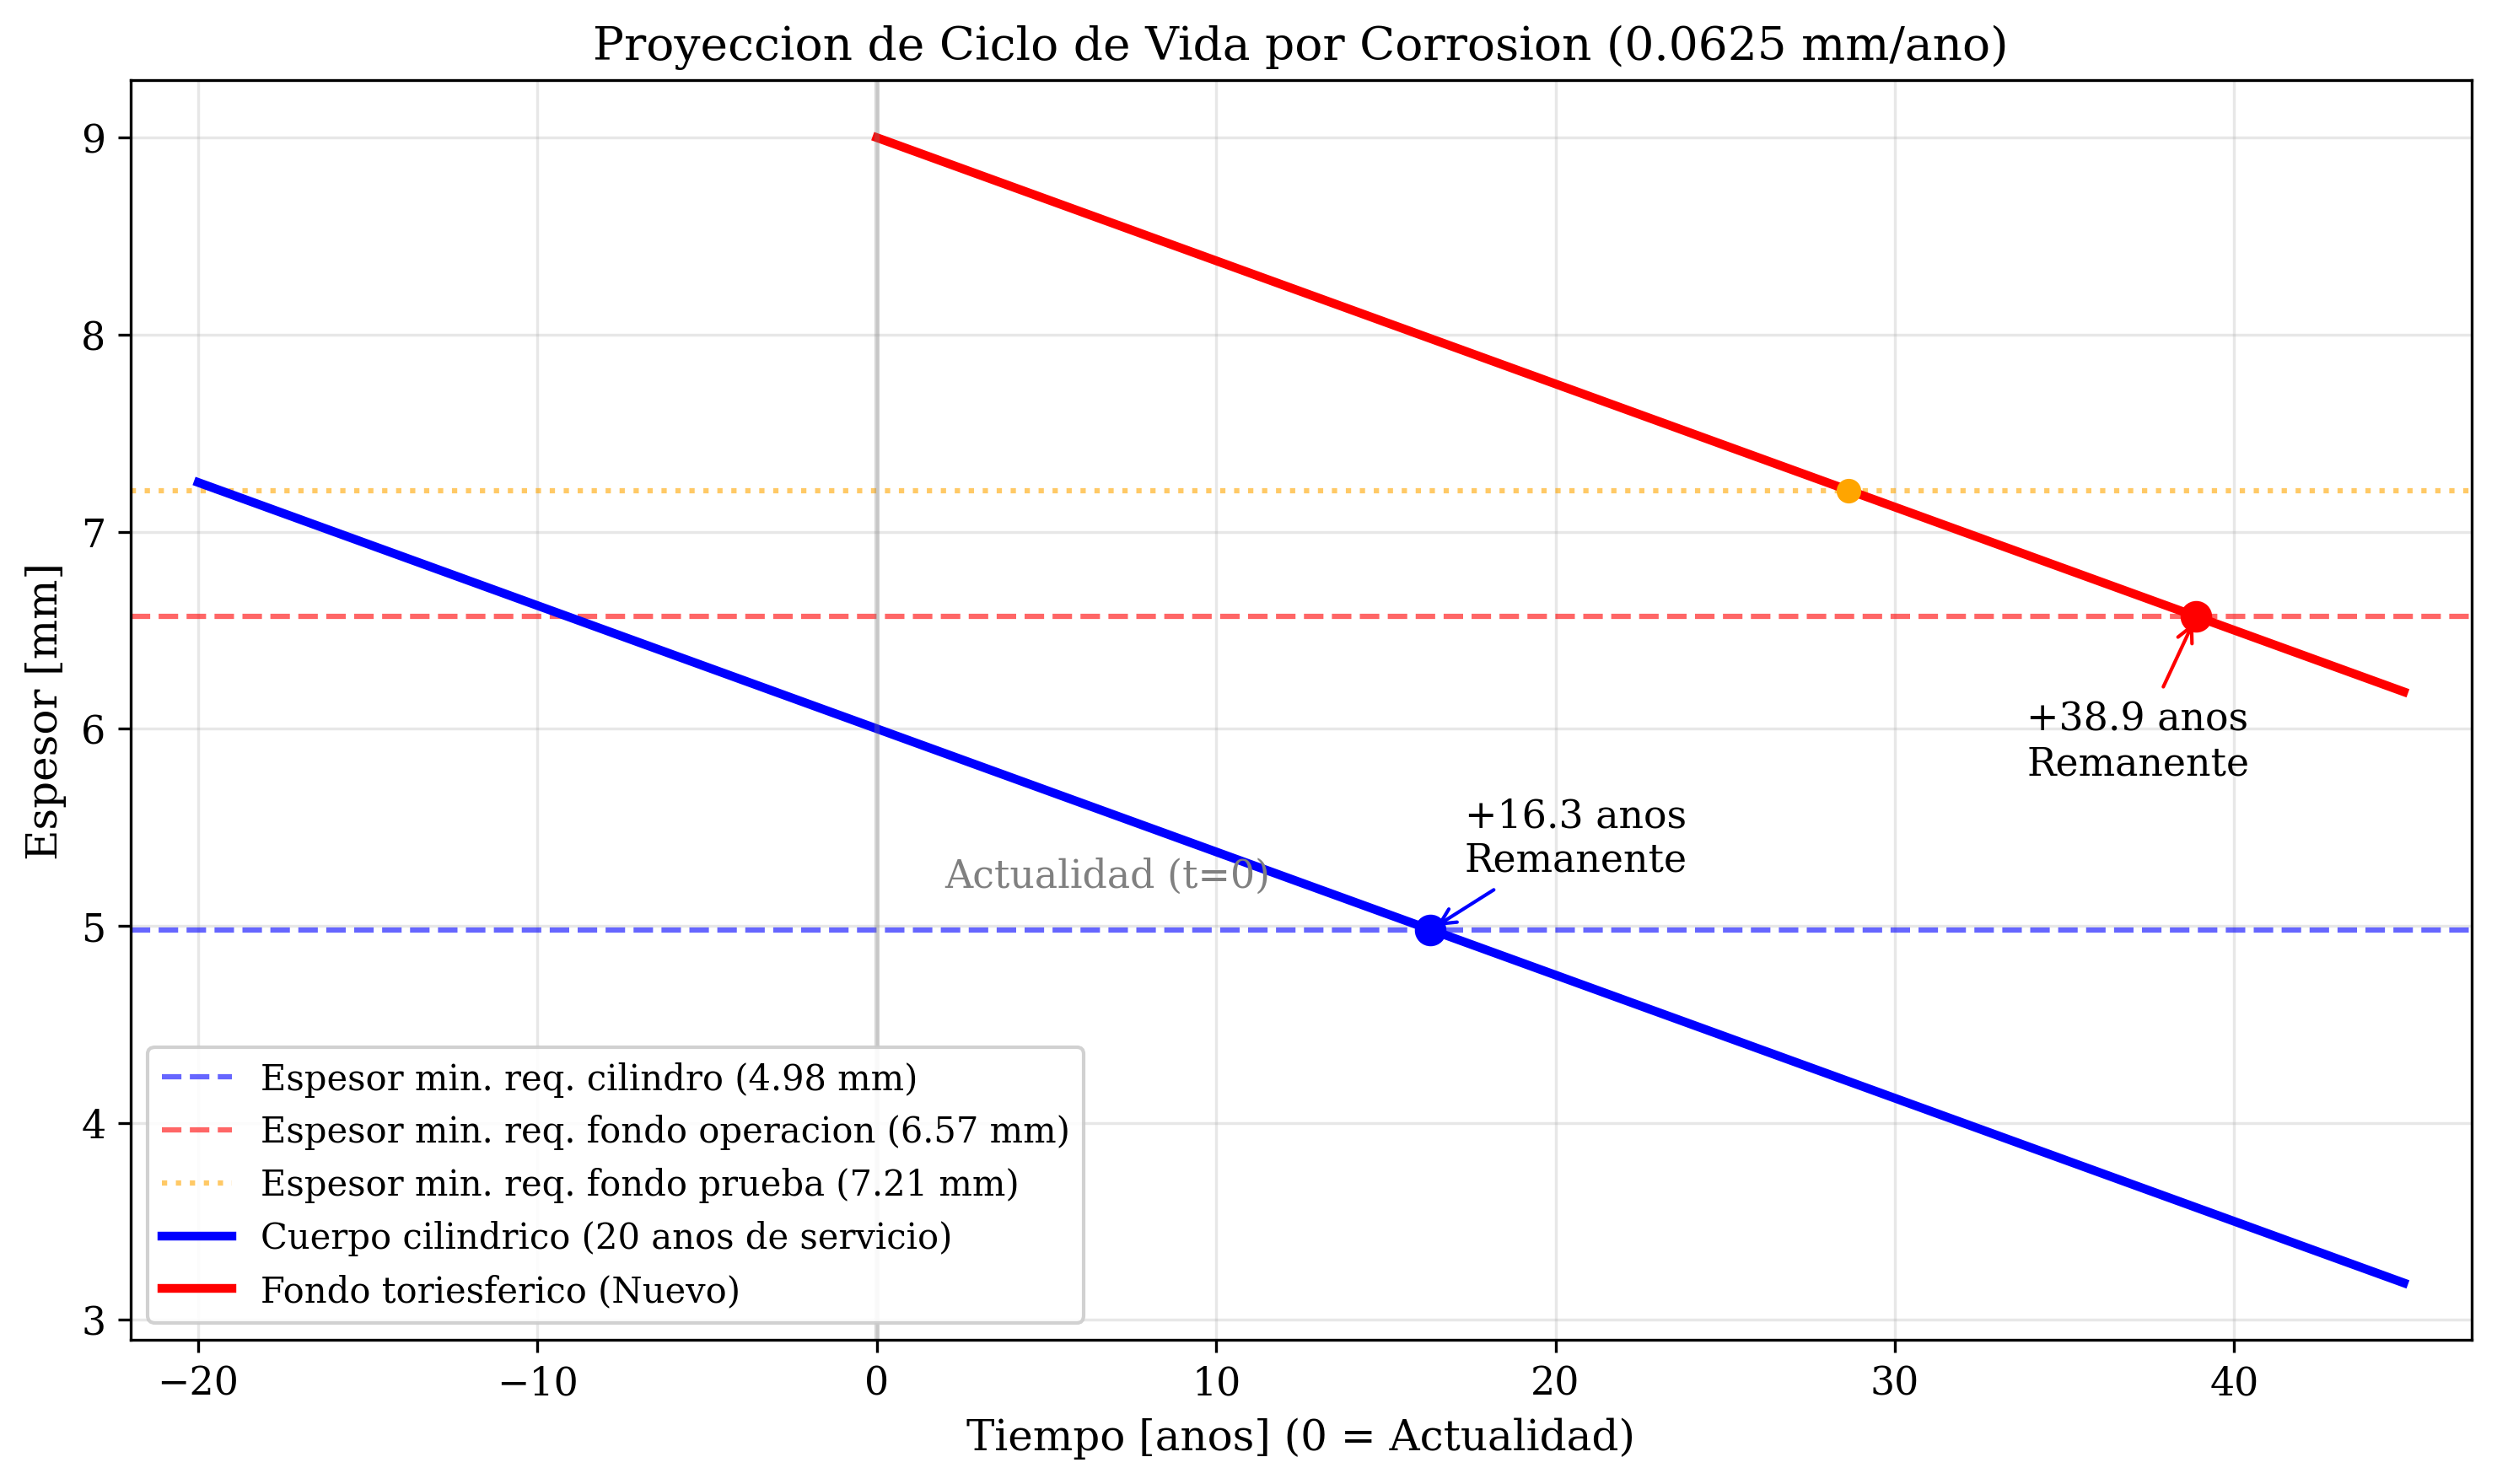
\includegraphics[width=0.85\textwidth]{../figures/ciclo_vida_corrosion.png}
	\caption{Proyección de degradación acelerada por Corrosión-Fatiga. El nuevo fondo alcanza su límite de diseño del 10\% a los 7.5 años debido a la interacción de la acidez, los 75°C y la alta ciclicidad operativa con una tasa de 0.12 mm/año.}
	\label{fig:ciclo_vida}
\end{figure}

El an\'alisis confirma un per\'iodo de operaci\'on seguro de al menos 16 a\~nos adicionales para la planta, condicionado al seguimiento e inspecci\'on por Mapeo de Corrosi\'on o l\'ineas de Phased Array Ultras\'onico (PAUT) dadas las uniones y gradientes de operaci\'on.

\subsubsection{Validaci\'on FEA --- ANSYS Mechanical}

La simulaci\'on de elementos finitos (FEA) del tanque se realiz\'o en ANSYS Mechanical para el caso de carga combinado de mayor severidad: carga hidrost\'atica de la columna de glucosa con el tanque completamente lleno (regiones c\'onica y cil\'indrica), m\'as la condici\'on t\'ermica de 75\,°C aplicada como frontera sobre la superficie interior del fondo toriesf\'erico. La Figura~\ref{fig:fea0} presenta la configuraci\'on del modelo con las condiciones de contorno activas. El cuerpo cil\'indrico aparece en gris, sin carga t\'ermica aplicada, mientras que el fondo toriesf\'erico se visualiza en rojo intenso, indicando la temperatura de 75\,°C impuesta sobre su superficie como condici\'on representativa del estado de calentamiento por la chaqueta de media ca\~na durante la operaci\'on.

\begin{figure}[H]
	\centering
	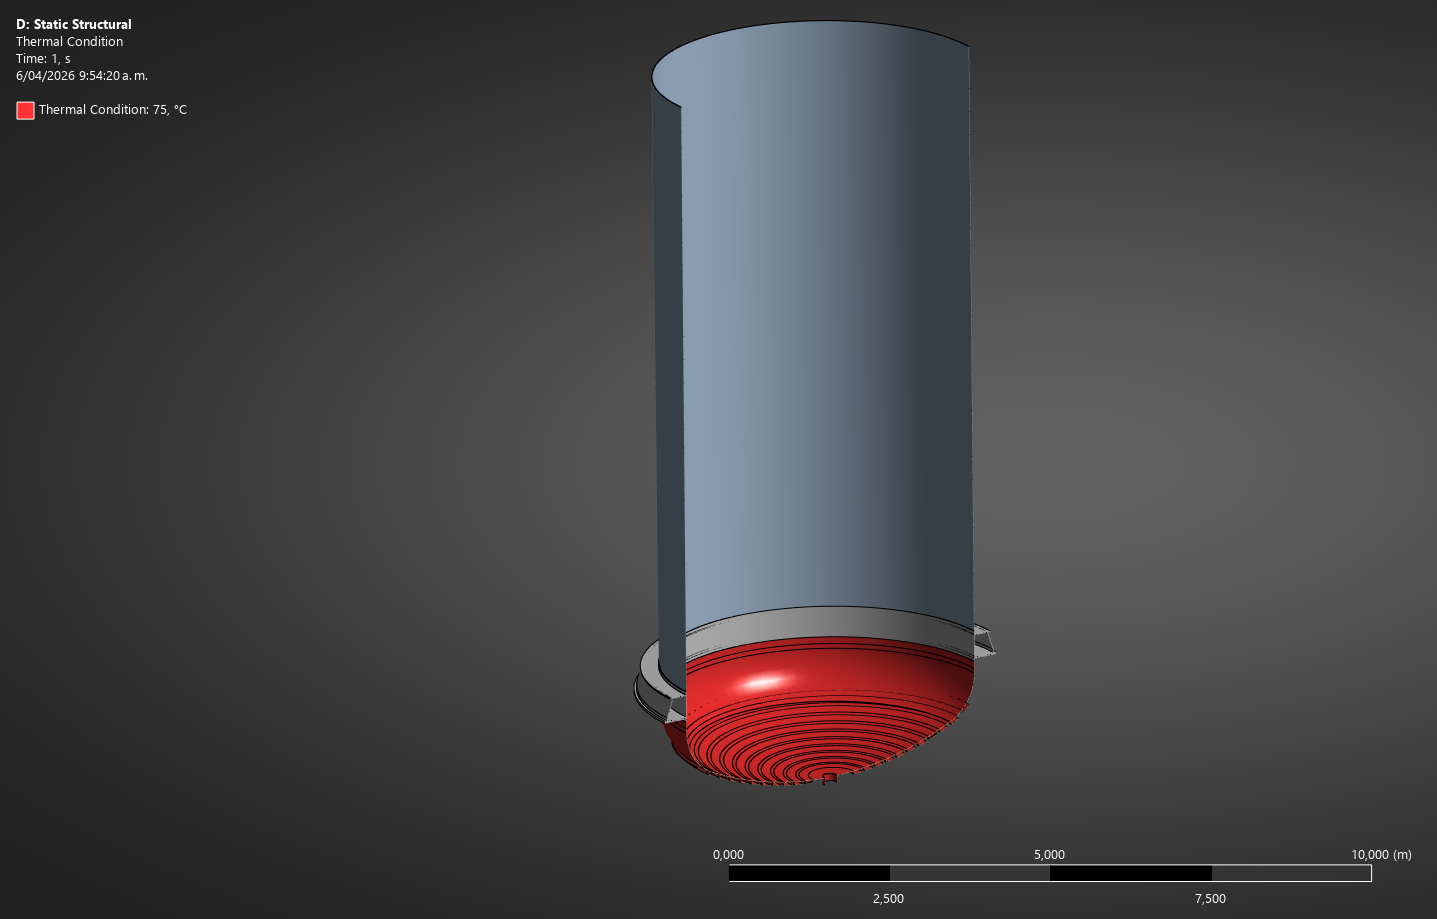
\includegraphics[width=0.72\textwidth]{../figures/fea0.png}
	\caption{Configuraci\'on del modelo FEA en ANSYS Mechanical. La condici\'on de temperatura de 75\,°C aplicada sobre el fondo toriesf\'erico se visualiza en rojo, mientras que el cuerpo cil\'indrico permanece sin carga t\'ermica. La chaqueta de media ca\~na en espiral y el anillo de soporte exterior se modelaron en su geometr\'ia real.}
	\label{fig:fea0}
\end{figure}

La Figura~\ref{fig:fea1} ilustra la distribuci\'on de la carga hidrost\'atica variable aplicada sobre la superficie interior del tanque. El gradiente crom\'atico de azul en la superficie libre (presi\'on nula) a rojo en la base del fondo toriesf\'erico (presi\'on m\'axima) reproduce fielmente la variaci\'on lineal de la presi\'on de la columna de glucosa con la profundidad. Esta distribuci\'on impone la mayor demanda estructural sobre el fondo toriesf\'erico y la virola inferior del cuerpo cil\'indrico, que son precisamente los componentes cr\'iticos identificados en el an\'alisis anal\'itico (Tabla~\ref{tab:espesores_fondo}).

\begin{figure}[H]
	\centering
	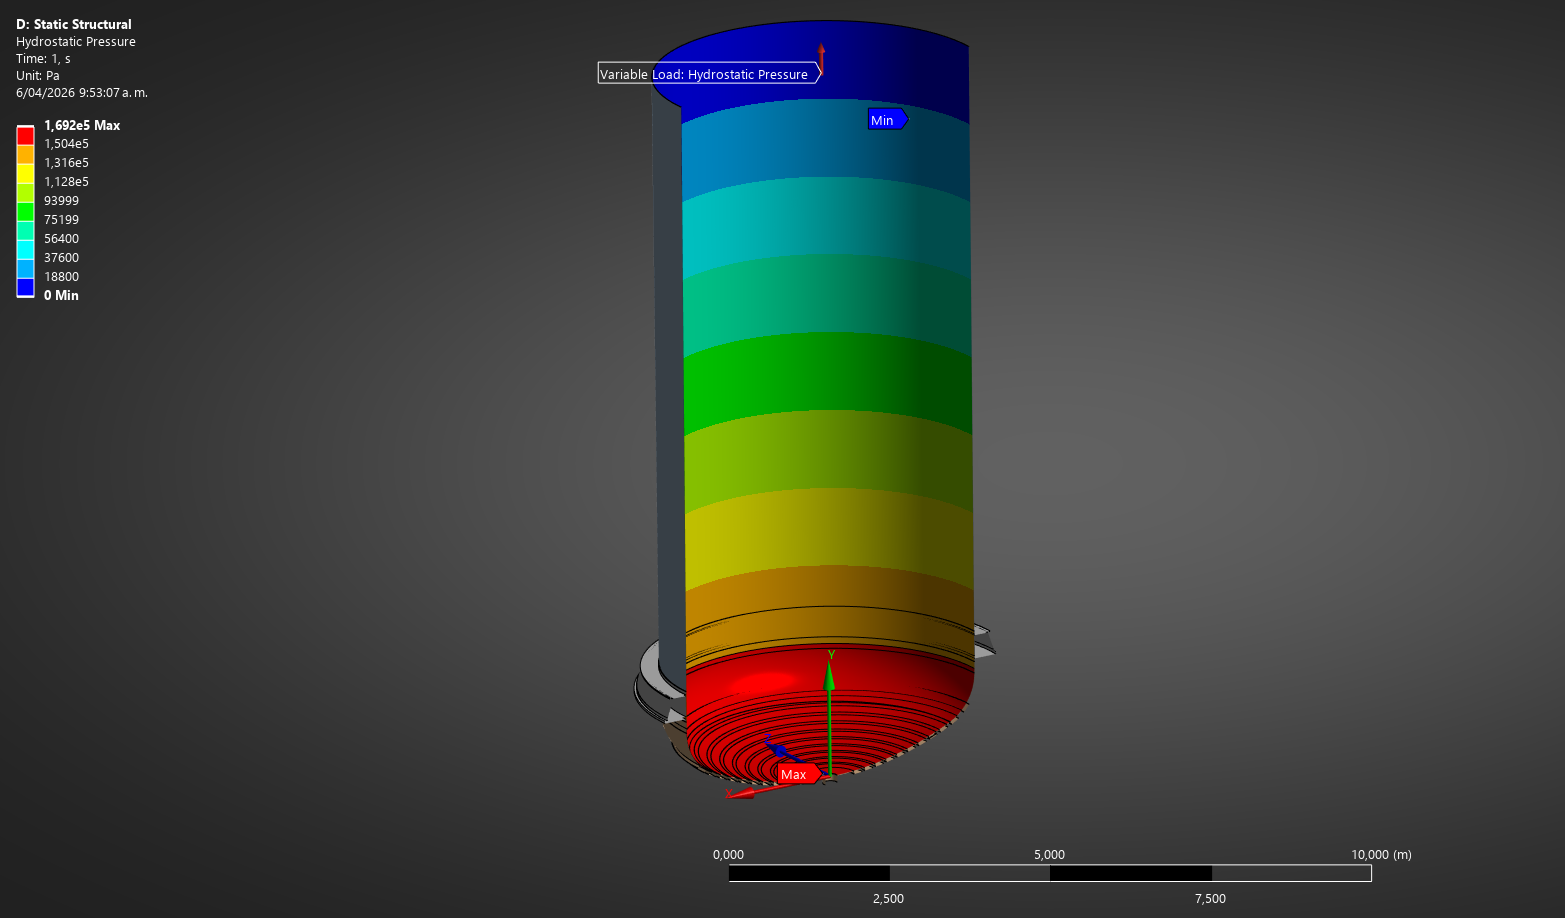
\includegraphics[width=0.72\textwidth]{../figures/fea1.png}
	\caption{Distribuci\'on de la carga hidrost\'atica variable (Variable Load: Hydrostatic Pressure) sobre el tanque lleno de glucosa. La escala crom\'atica var\'ia de azul en la superficie libre (presi\'on nula) a rojo en la base del fondo toriesf\'erico (presi\'on m\'axima), reflejando la variaci\'on lineal de presi\'on con la profundidad.}
	\label{fig:fea1}
\end{figure}

La Figura~\ref{fig:fea2} presenta la distribuci\'on del esfuerzo equivalente de Von Mises sobre el fondo toriesf\'erico (vista ampliada con malla visible). El resultado revela con claridad los dos focos de concentraci\'on de esfuerzos m\'as significativos del sistema: la zona de transici\'on fondo-cil\'indro (nudillo), donde la geometr\'ia curva del fondo toriesf\'erico se une al cuerpo cil\'indrico mediante una curvatura de menor radio, y los puntos de anclaje de la chaqueta de media ca\~na al fondo, donde la soldadura genera discontinuidades geom\'etricas y, en consecuencia, concentradores de esfuerzo locales. Ambas zonas exhiben tonos naranja y amarillo, indicando esfuerzos notablemente superiores a los del centro del fondo (tonos verde y azul), donde la geometr\'ia toriesf\'erica distribuye la carga de manera m\'as uniforme.

\begin{figure}[H]
	\centering
	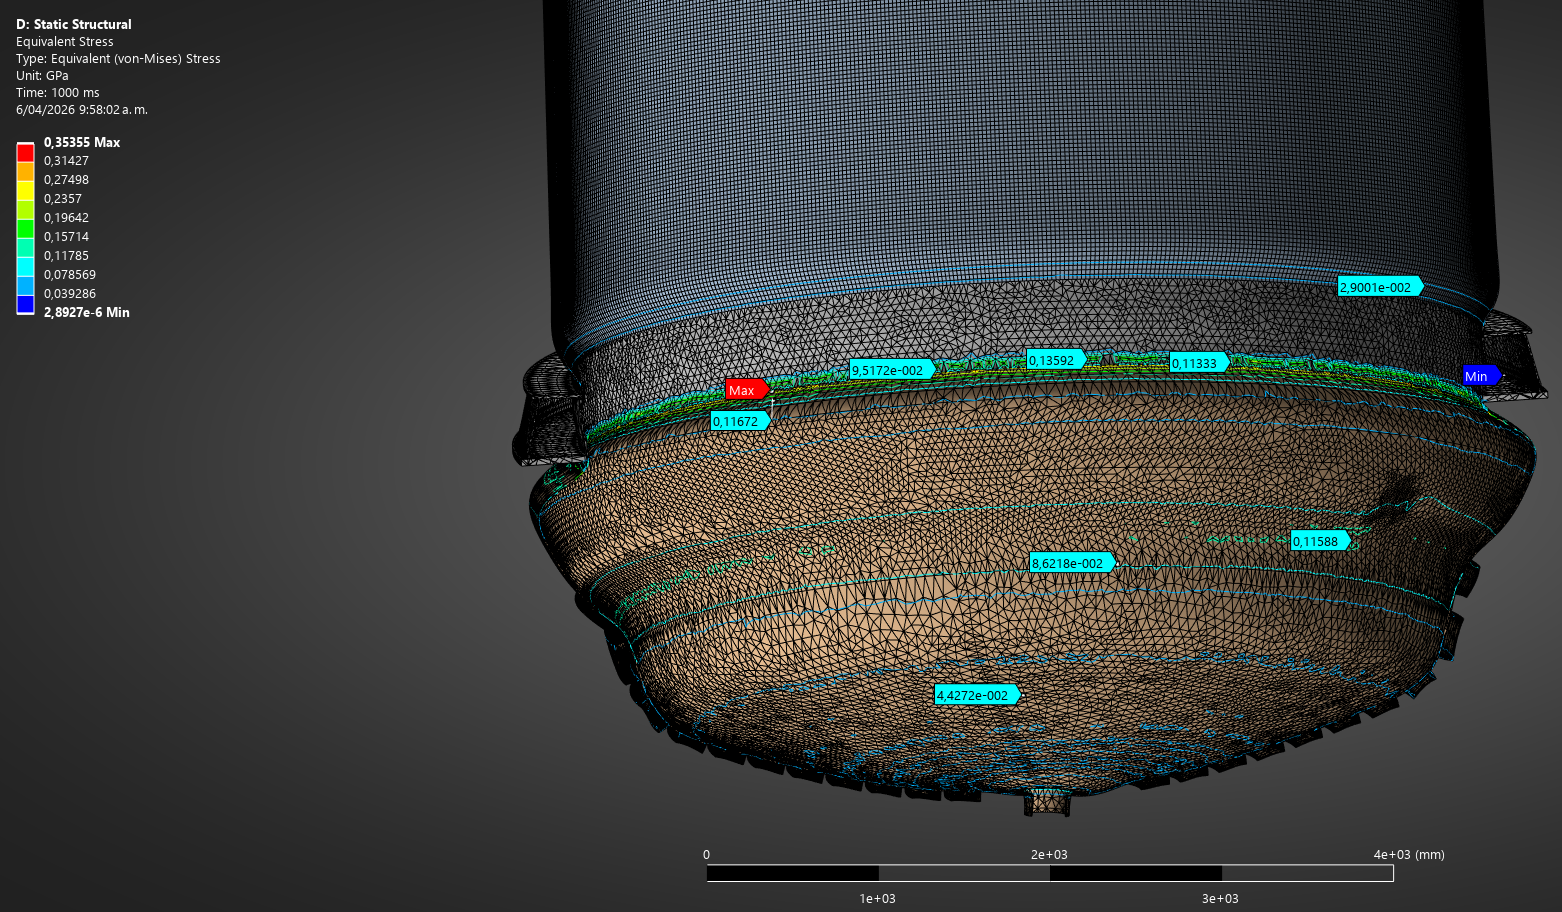
\includegraphics[width=0.85\textwidth]{../figures/fea2.png}
	\caption{Distribuci\'on del esfuerzo equivalente de Von Mises sobre el fondo toriesf\'erico (vista acercada con malla visible). Los mayores esfuerzos se concentran en la zona de transici\'on fondo-cil\'indro (nudillo) y en los puntos de soldadura de la chaqueta de media ca\~na (tonos naranja y amarillo), mientras que el centro del fondo presenta niveles de esfuerzo moderados (verde/azul).}
	\label{fig:fea2}
\end{figure}

La Figura~\ref{fig:fea3} presenta el resultado de mayor relevancia estructural del estudio: la distribuci\'on del factor de seguridad sobre el ensamble fondo-chaqueta bajo la carga combinada t\'ermica e hidrost\'atica. Las zonas en verde corresponden a factores de seguridad superiores a 2, que representan condiciones estructuralmente satisfactorias. Las zonas en amarillo y naranja exhiben factores marginales en el rango de 1 a 2. De particular atenci\'on son las zonas de color rojo, localizadas espec\'ificamente en el nudillo fondo-cil\'indro y en los puntos de anclaje de la chaqueta de media ca\~na, donde el factor de seguridad desciende a un m\'inimo de aproximadamente 0.71. Un factor de seguridad inferior a la unidad implica que el esfuerzo local supera el esfuerzo admisible del SS316L ($S = 115$~MPa a 75\,°C, ASME~Section~II~Part~D) bajo la carga combinada aplicada, constituyendo una condici\'on de sobreesfuerzo local que requiere atenci\'on de dise\~no. Este hallazgo es plenamente consistente con la conclusi\'on del an\'alisis anal\'itico, que determin\'o que el fondo toriesf\'erico opera al l\'imite de su espesor nominal al 100\% de llenado y no cumple el requisito ASME~VIII en esa condici\'on (Tabla~\ref{tab:espesores_fondo}).

\begin{figure}[H]
	\centering
	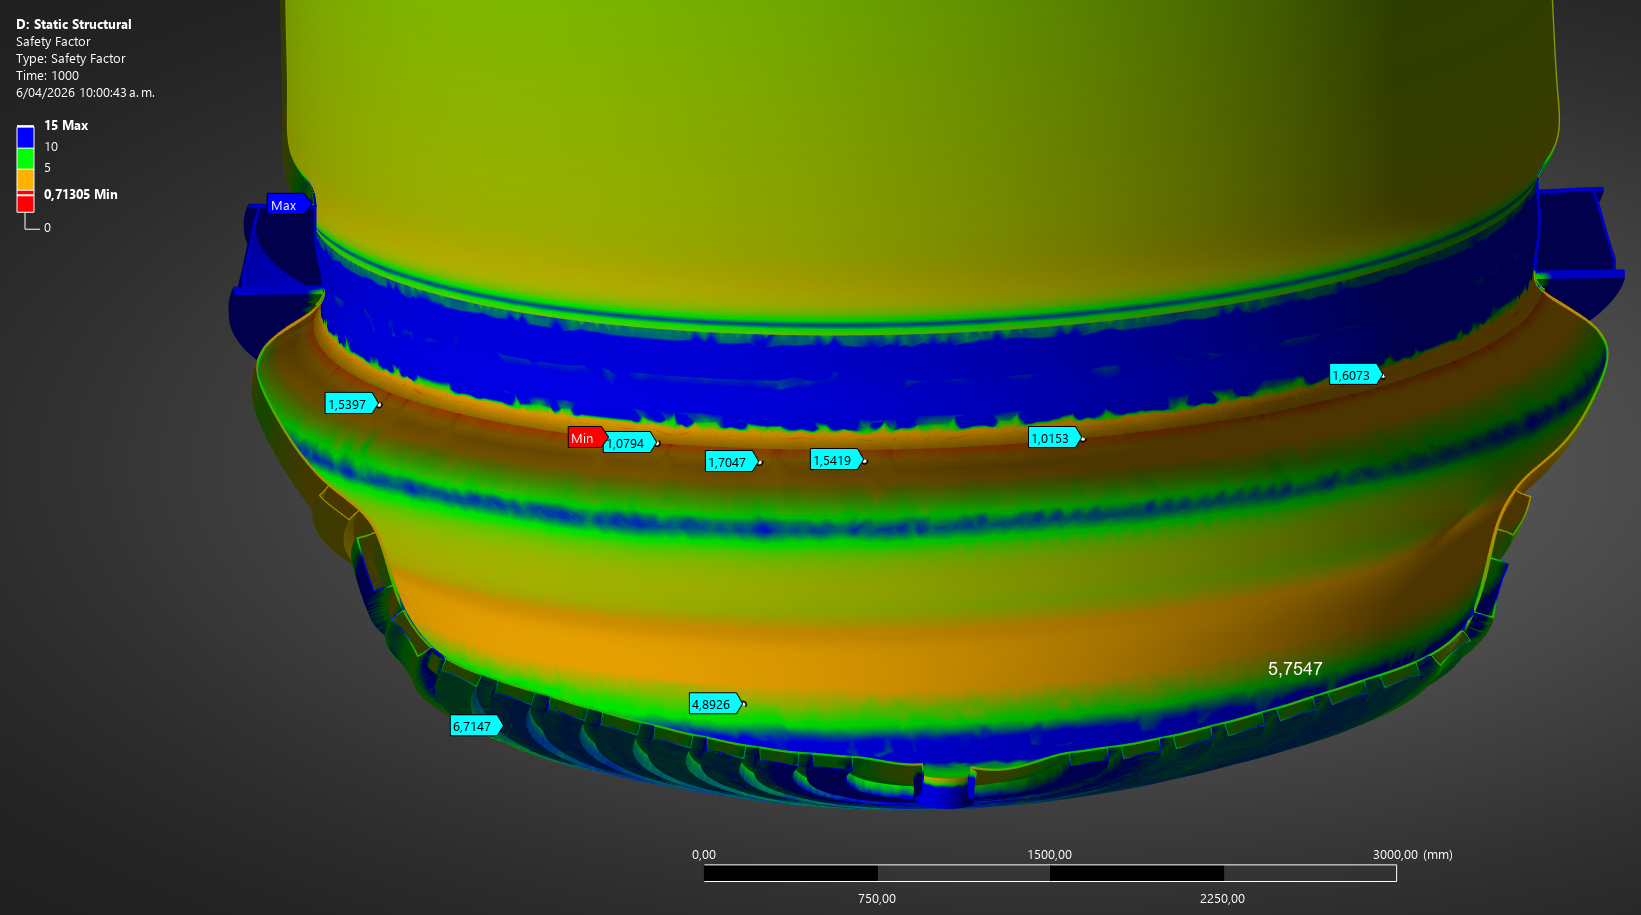
\includegraphics[width=0.85\textwidth]{../figures/fea3.png}
	\caption{Distribuci\'on del factor de seguridad sobre el fondo toriesf\'erico y la chaqueta de media ca\~na bajo carga combinada (hidrost\'atica + t\'ermica 75\,°C). Las zonas en rojo presentan factores de seguridad inferiores a la unidad ($FS_{\min} \approx 0.71$), localizados en el nudillo fondo-cil\'indro y en los puntos de soldadura de la chaqueta, confirmando el sobreesfuerzo local bajo la condici\'on de llenado al 100\%.}
	\label{fig:fea3}
\end{figure}

La Figura~\ref{fig:fea4} muestra la distribuci\'on de deformaci\'on total del sistema bajo la carga combinada. El patr\'on de deformaci\'on es sim\'etrico y responde al comportamiento esperado de un cabezal a presi\'on interna con carga t\'ermica diferencial: la deflexión m\'axima de aproximadamente 4.1~mm ocurre en el punto geom\'etricamente m\'as expuesto, es decir, el centro del fondo toriesf\'erico, como resultado de la superposici\'on de la presi\'on hidrost\'atica y la expansi\'on t\'ermica diferencial inducida por la temperatura de 75\,°C en el fondo frente al cuerpo cil\'indrico sin calefacci\'on. La deformaci\'on decrece radialmente hacia la periferia del fondo, alcanzando valores m\'inimos en el anillo de soporte exterior, donde la condici\'on de apoyo sobre la losa de concreto restringe el desplazamiento. Este patr\'on no indica por s\'i solo un riesgo estructural cr\'itico, pero es un par\'ametro relevante para la evaluaci\'on de los sistemas de tuber\'ias y conexiones flexibles vinculadas al fondo.

\begin{figure}[H]
	\centering
	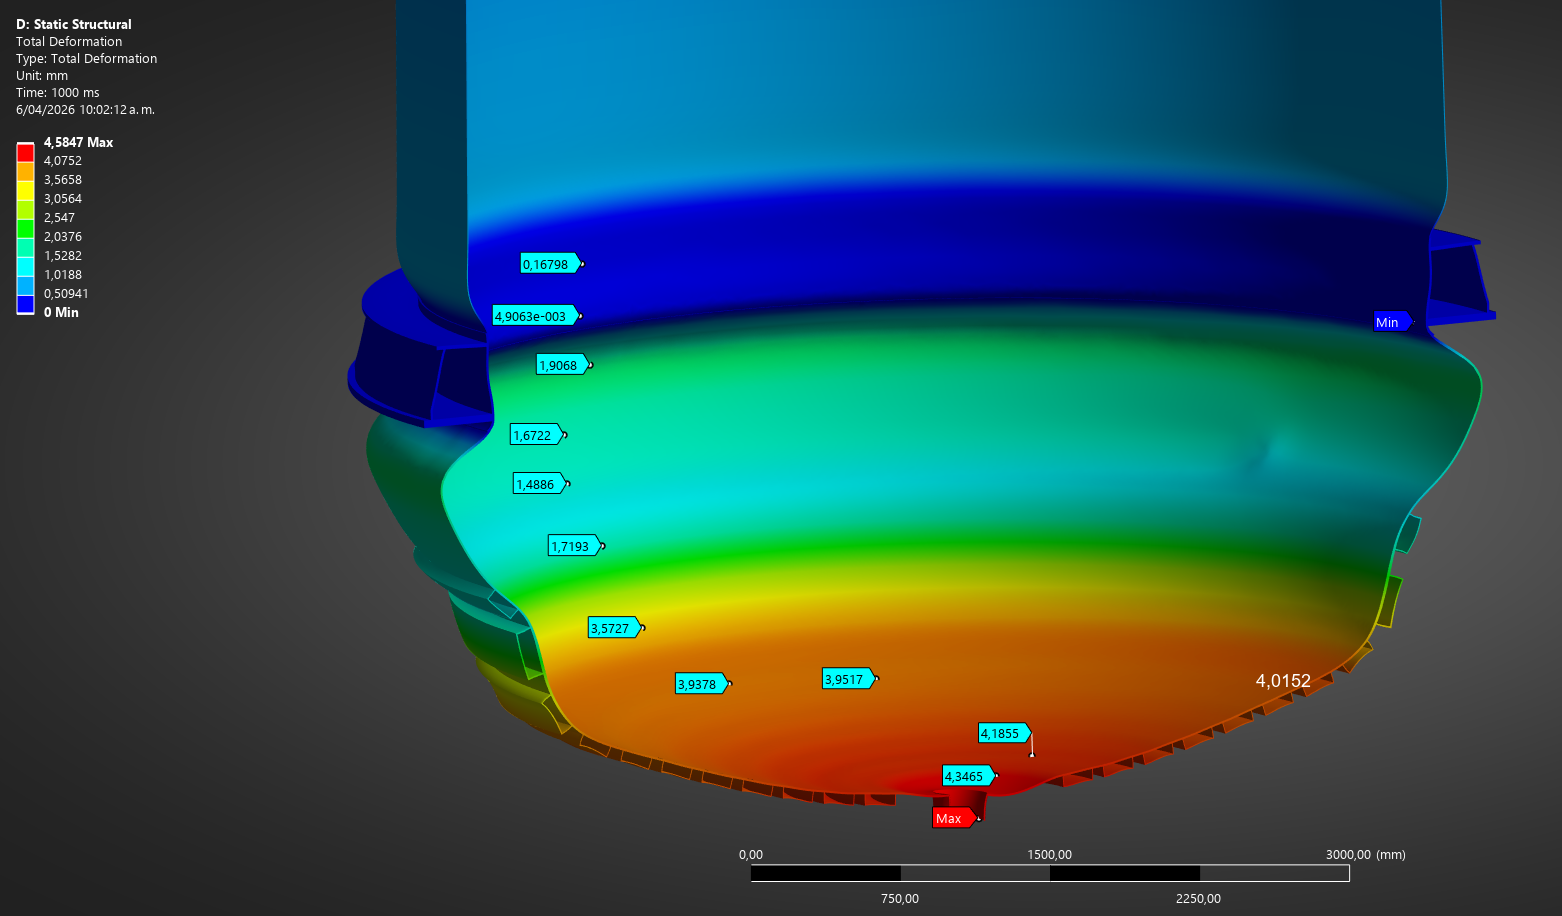
\includegraphics[width=0.85\textwidth]{../figures/fea4.png}
	\caption{Distribuci\'on de deformaci\'on total bajo carga combinada (hidrost\'atica + t\'ermica 75\,°C). La deflexión m\'axima de $\approx\!4.1$~mm se localiza en el centro del fondo toriesf\'erico. La deformaci\'on decrece radialmente hacia el anillo de soporte (desplazamiento m\'inimo), con un patr\'on sim\'etrico consistente con el comportamiento de un cabezal bajo presi\'on interna con gradiente t\'ermico.}
	\label{fig:fea4}
\end{figure}

\newpage
